% =============================================================================
% FILE NAME : thesis.tex
% DEPARTMENT: University of Tuebingen
% AUTOR     : Paul Palomero Bernardo & Konstantin Lübeck
% =============================================================================
% CONTENT   : LaTeX header file for master's thesis
% =============================================================================
% Documentclass and packages
% =============================================================================
\documentclass[oneside,11pt,a4paper,twoside]{scrreprt}
\usepackage[left=3cm, right=3cm,top=3cm,bottom=3.5cm]{geometry}
\usepackage{xspace}[2006/05/08]
\xspaceaddexceptions{])\}}
\usepackage[backend=biber, style=ieee, url=false, doi=false, isbn=false]{biblatex}
\usepackage{scrhack}
\usepackage[utf8]{inputenc}
\usepackage[T1]{fontenc}
\usepackage[autostyle]{csquotes}
\usepackage[ngerman,english]{babel}
\usepackage{mathtools}
\usepackage{amsmath}
\usepackage{amssymb}
\usepackage{amsfonts}
\usepackage{amsthm}
\usepackage{lmodern}
\usepackage[table]{xcolor}
\usepackage{graphicx}
\usepackage{verbatim}
\usepackage[margin=10pt,font=small,labelfont=bf]{caption}
\usepackage{subcaption}
\usepackage{listings}
\usepackage{algorithm}
\usepackage[noend]{algpseudocode}
\usepackage{paralist}
\usepackage{booktabs}
\usepackage{multirow}
\usepackage{siunitx}
\usepackage{pifont}
\usepackage{lscape}
\usepackage{enumitem}
\usepackage{setspace}
\usepackage[toc,acronym,nonumberlist,automake,nopostdot,nogroupskip]{glossaries}
\usepackage{todonotes}
\usepackage{pgfplots}
\usepackage[usenames,dvipsnames]{pstricks}
\usepackage{epsfig}
\usepackage{rotating}
\usepackage{changepage}
\usepackage[noabbrev]{cleveref}
\usepackage{ifthen}
\usepackage{blindtext}
% =============================================================================
% Custom commands
% =============================================================================
% =============================================================================
% Page margin and header setup
% =============================================================================
\textwidth 14cm
\textheight 22cm
\topmargin 0.0cm
\evensidemargin 1cm
\oddsidemargin 1cm
\pagestyle{headings}
\clubpenalty10000
\widowpenalty10000
\displaywidowpenalty=10000
\parskip 0.5ex plus 0.1ex minus 0.1ex
% =============================================================================
% Package setup
% =============================================================================
% === Array ===
\renewcommand{\arraystretch}{1.3}
% === Graphicx ===
\graphicspath{{images/}}
% === Biblatex ===
\addbibresource{includes/bibliography.bib}
\AtEveryBibitem{%
	\clearlist{language}%
}
% === Glossaries ===
\makeglossaries
\renewcommand{\glossarypreamble}{\glsfindwidesttoplevelname[\currentglossary]}
% === Algpseudocode ===
\newcommand{\algorithmautorefname}{Algorithm}
\algrenewcommand{\algorithmiccomment}[1]{\hfill\textit{#1}}
\algdef{S}[FOR]{LFor}[2]{\textit{#1:}\ \algorithmicfor\ #2\ \algorithmicdo}
% === Pgfplots ===
\pgfplotsset{compat=newest}
% === Amsthm ===
\theoremstyle{definition}
\newtheorem{defn}{Definition}[chapter]
\newtheorem{thm}[defn]{Satz}
\newtheorem{analysis}{Analyse}[chapter]
\theoremstyle{remark}
\newtheorem{exmp}[defn]{Beispiel}
\newtheorem*{note}{Bemerkung}
% === xcolor ===
\definecolor{universityred}{RGB}{165,30,55}
\definecolor{customblue}{RGB}{54,75,154}
\definecolor{customorange}{RGB}{246,126,75}
\definecolor{customred}{RGB}{165,0,38}
\definecolor{customneutral}{RGB}{254,218,139}
% === Listings ===
\renewcommand{\lstlistingname}{Codeauszug}
\renewcommand{\lstlistlistingname}{Codeauszugsverzeichnis}
\lstset{literate=%
    {Ö}{{\"O}}1
    {Ä}{{\"A}}1
    {Ü}{{\"U}}1
    {ß}{{\ss}}1
    {ü}{{\"u}}1
    {ä}{{\"a}}1
    {ö}{{\"o}}1
    {~}{{\textasciitilde}}1
}
\lstdefinestyle{customc}{
    framextopmargin=1pt,
    framexbottommargin=1pt, 
    frame=tb, 
    framerule=0.7pt,
    belowcaptionskip=1\baselineskip,
    breaklines=true,
    language=C,
    tabsize=2,
    showstringspaces=false,
    basicstyle=\tiny\ttfamily,
    %backgroundcolor=\color{customlightgray},
    keywordstyle=\bfseries\color{customlightred},
    commentstyle=\color{customblue},
    identifierstyle=\color{customgreen},
    stringstyle=\color{orange},
    moredelim=[s][\color{ForestGreen}\sffamily]{/**}{*/},
    moredelim=[l][\color{customblue}]{\#pragma}
}
% =============================================================================
% Variable declarations
% =============================================================================

% true = english
% false = german
\newboolean{english}
\setboolean{english}{false}

\def\authorsurname{TODO: SURNAME}
\def\authorfirstname{TODO: FIRST NAME}
\def\title{TODO: TITLE}
\def\thesiskind{Master's Thesis}
\def\thesisstart{TODO: START DATE}
\def\thesisend{TODO: END DATE}
% =============================================================================
% siunitx
% =============================================================================
\sisetup{locale = UK}
\sisetup{detect-all = true}
\sisetup{per-mode = symbol}
\DeclareSIUnit\op{OP}
\DeclareSIUnit\ops{OPS}
\DeclareSIUnit\mac{MAC}
\DeclareSIUnit\macs{MACS}
\DeclareSIUnit\cycle{cycle}
% =============================================================================
% symbols
% =============================================================================
\newcommand{\cmark}{\ding{51}}%
\newcommand{\xmark}{\ding{55}}%
% =============================================================================
% tabular
% =============================================================================
\newcommand{\rowgray}{\rowcolor[gray]{.9}}%
% =============================================================================
% mathtools: equation numbering style
% =============================================================================
\renewcommand{\theequation}{\arabic{chapter}.\arabic{equation}}
\newtagform{bold}[\textbf]{}{}
\usetagform{bold}
% =============================================================================
% enumitem
% =============================================================================
\setitemize{itemsep=0.15em, topsep=0.5em}
\setenumerate{itemsep=0.15em, topsep=0.5em}

% =============================================================================
% FILE NAME : abbreviations.tex
% DEPARTMENT: University of Tuebingen
% AUTOR     : Paul Palomero Bernardo
% =============================================================================
% CONTENT   : Include for abbreviations
% =============================================================================
\newacronym{mlp}{MLP}{multilayer perceptron}

% =============================================================================
% DOCUMENT START
% =============================================================================
\begin{document}
% =============================================================================
% Titlepage
% =============================================================================
\ifthenelse{\boolean{english}}{
	\newgeometry{top=2.7cm}
	\begin{titlepage}
		\begin{adjustwidth}{-1cm}{-1cm}
		\begin{minipage}{0.5\textwidth}
			
\includegraphics[width=\linewidth]{figures/logo.pdf}
		\end{minipage}
		\hfill
		\begin{minipage}{0.3\textwidth}
			{\bfseries\textsf{\textcolor{universityred}{Faculty of\\Science}}\\[0.3cm]}
			{\bfseries\textsf{\textcolor{universityred}{Embedded Systems}}}
		\end{minipage}%
		\end{adjustwidth}
		\vspace{3cm}
		\begin{center}
			{\huge \thesiskind\\[2cm]}
			{\Large\bfseries \title\\[1.5cm]}
			{\large Submitted by: \authorfirstname\ \authorsurname}\\[0.5cm]
			\thesisend
		\end{center}
		\vfill
		\begin{minipage}{0.48\textwidth}
			\centering
			{\small\bfseries First Supervisor}\\[0.3cm]
			{\large Prof. Dr. Oliver Bringmann}\\[2mm]
			{\footnotesize Faculty of Science\\
			Department of Computer Science\\[1.5mm]
			Embedded Systems\\
			University of Tübingen}
		\end{minipage}
		\hfill
		\begin{minipage}{0.48\textwidth}
			\centering
			{\small\bfseries Second Supervisor}\\[0.3cm]
			{\large TODO: NAME}\\[2mm]
			{\footnotesize Faculty of Science\\
			Department of Computer Science\\[1.5mm]
			TODO: CHAIR\\
			University of Tübingen}
		\end{minipage}%
		\vspace{1.5cm}
		\begin{minipage}{0.48\textwidth}
			\centering
			{\small\bfseries Graduate Advisor}\\[0.3cm]
			{\large TODO: NAME}\\[2mm]
			{\footnotesize Faculty of Science\\
				Department of Computer Science\\[1.5mm]
				Embedded Systems\\
				University of Tübingen}
		\end{minipage}
		\hfill
		\begin{minipage}{0.48\textwidth}
			\centering
			{\small\bfseries Graduate Advisor}\\[0.3cm]
			{\large TODO: NAME}\\[2mm]
			{\footnotesize Faculty of Science\\
				Department of Computer Science\\[1.5mm]
				Embedded Systems\\
				University of Tübingen}
		\end{minipage}
	\end{titlepage}
}{
	\newgeometry{top=2.7cm}
	\begin{titlepage}
		\begin{adjustwidth}{-1cm}{-1cm}
		\begin{minipage}{0.5\textwidth}
			
\includegraphics[width=\linewidth]{figures/logo.pdf}
		\end{minipage}
		\hfill
		\begin{minipage}{0.4\textwidth}
			{\bfseries\textsf{\textcolor{universityred}{Mathematisch-\\Naturwissenschaftliche Fakultät}}\\[0.3cm]}
			{\bfseries\textsf{\textcolor{universityred}{Eingebettete Systeme}}}
		\end{minipage}%
		\end{adjustwidth}
		\vspace{3cm}
		\begin{center}
			{\huge \thesiskind\\[2cm]}
			{\Large\bfseries \title\\[1.5cm]}
			{\large \authorfirstname\ \authorsurname}\\[0.5cm]
			\thesisend
		\end{center}
		\vfill
		\begin{minipage}{0.48\textwidth}
			\centering
			{\small\bfseries Erster Gutachter}\\[0.3cm]
			{\large Prof. Dr. Oliver Bringmann}\\[2mm]
			{\footnotesize Mathematisch-Naturwissenschaftliche\\Fakultät\\
			Fachbereich Informatik\\[1.5mm]
			Lehrstuhl Eingebettete Systeme\\
			Universität Tübingen}
		\end{minipage}
		\hfill
		\begin{minipage}{0.48\textwidth}
			\centering
			{\small\bfseries Zweiter Gutachter}\\[0.3cm]
			{\large TODO: NAME}\\[2mm]
			{\footnotesize Mathematisch-Naturwissenschaftliche\\Fakultät\\
			Fachbereich Informatik\\[1.5mm]
			TODO: LEHRSTUHL\\
			Universität Tübingen}
		\end{minipage}%
		\vspace{1.5cm}
		\begin{minipage}{0.48\textwidth}
			\centering
			{\small\bfseries Betreuer}\\[0.3cm]
			{\large TODO: NAME}\\[2mm]
			{\footnotesize Mathematisch-Naturwissenschaftliche\\Fakultät\\
			Fachbereich Informatik\\[1.5mm]
			Lehrstuhl Eingebettete Systeme\\
			Universität Tübingen}
		\end{minipage}
		\hfill
		\begin{minipage}{0.48\textwidth}
			\centering
			{\small\bfseries Betreuer}\\[0.3cm]
			{\large TODO: NAME}\\[2mm]
			{\footnotesize Mathematisch-Naturwissenschaftliche\\Fakultät\\
			Fachbereich Informatik\\[1.5mm]
			Lehrstuhl Eingebettete Systeme\\
			Universität Tübingen}
		\end{minipage}
	\end{titlepage}
}
% =============================================================================
% 2nd page: Titlepage
% =============================================================================
\thispagestyle{empty}
\vspace*{\fill}
\noindent
\begin{minipage}{.8\textwidth}
	\textbf{\authorsurname, \authorfirstname:}\\
	\emph{\title}\\
	\thesiskind\\
	\ifthenelse{\boolean{english}}{
		University of Tübingen\\
		Processing period: \thesisstart\ - \thesisend
	}{
		Eberhard Karls Universität Tübingen\\
		Bearbeitungszeitraum: \thesisstart\ - \thesisend
	}
\end{minipage}
\cleardoublepage

% =============================================================================
% Abstract
% =============================================================================
\begin{onehalfspace}
\ifthenelse{\boolean{english}}{
	\chapter*{Kurzfassung}
	\thispagestyle{empty}
	\begin{otherlanguage}{ngerman}
		% =============================================================================
% FILE NAME : abstractger.tex
% DEPARTMENT: University of Tuebingen
% AUTOR     : Paul Palomero Bernardo
% =============================================================================
% CONTENT   : Include for abstract (german)
% =============================================================================
Obwohl diese Arbeit in Englisch verfasst wird muss es einen deutschen Abstract/Kurzfassung geben. (Übersetzung des englischen Abstracts)

	\end{otherlanguage}
	\cleardoublepage
	\chapter*{Abstract}
	\thispagestyle{empty}
	% =============================================================================
% FILE NAME : abstract.tex
% DEPARTMENT: University of Tuebingen
% AUTOR     : Tom Schammo
% =============================================================================
% CONTENT   : Include for abstract (english)
% =============================================================================

This thesis sets out to implement keyword-spotting on the UltraTrail architecture.
To that end, different input sources are implemented and analyzed.
An additional goal is to extend the Rust ecosystem by adding support for UltraTrail to Rust.
To achieve this, UltraTrail is added to the PAC and its drivers are implemented in the HAL.
The $I^2S$ and PDM driver implementations are then tested.
Testing reveals that the microphone drivers do not work as expected and despite
resolving some issues, it was not possible to get the microphones to work as desired,
so keyword-spotting could not be implemented.
However, the UltraTrail driver has been successfully implemented and tested so that
future research can be conducted on the effectiveness of keyword-spotting on the UltraTrail.

	\cleardoublepage
}{
	\chapter*{Kurzfassung}
	\thispagestyle{empty}
	% =============================================================================
% FILE NAME : abstract.tex
% DEPARTMENT: University of Tuebingen
% AUTOR     : Tom Schammo
% =============================================================================
% CONTENT   : Include for abstract (english)
% =============================================================================

This thesis sets out to implement keyword-spotting on the UltraTrail architecture.
To that end, different input sources are implemented and analyzed.
An additional goal is to extend the Rust ecosystem by adding support for UltraTrail to Rust.
To achieve this, UltraTrail is added to the PAC and its drivers are implemented in the HAL.
The $I^2S$ and PDM driver implementations are then tested.
Testing reveals that the microphone drivers do not work as expected and despite
resolving some issues, it was not possible to get the microphones to work as desired,
so keyword-spotting could not be implemented.
However, the UltraTrail driver has been successfully implemented and tested so that
future research can be conducted on the effectiveness of keyword-spotting on the UltraTrail.

	\cleardoublepage
}
\end{onehalfspace}

% =============================================================================
% Acknowledgements 
% =============================================================================
\begin{onehalfspace}
\ifthenelse{\boolean{english}}
	{\chapter*{Acknowledgements}}
	{\chapter*{Danksagung}}
\thispagestyle{empty}
Danksagung (falls gewünscht)
\cleardoublepage
\end{onehalfspace}

% =============================================================================
% Table of contents
% =============================================================================
% page numbering setup
\pagenumbering{Roman}
\setcounter{page}{1}
\pagestyle{headings}
\renewcommand{\baselinestretch}{1.3}
\small\normalsize
\tableofcontents
\renewcommand{\baselinestretch}{1}
\small\normalsize
\cleardoublepage
% =============================================================================
% Page numbering setup
% =============================================================================
\pagenumbering{arabic}
\setcounter{page}{1}

% =============================================================================
% Chapters
% =============================================================================
\begin{onehalfspace}
\ifthenelse{\boolean{english}}
	{\chapter{Introduction}}
	{\chapter{Einleitung}}
\label{cha:introduction}
% =============================================================================
% FILE NAME : 00_introduction.tex
% DEPARTMENT: University of Tuebingen
% AUTOR     : Tom Schammo
% =============================================================================
% CONTENT   : Include for chapter "Introduction"
% =============================================================================

Rust \cite{rustlang} is a somewhat new language, with its very first release in early 2012.
But the 1.0 alpha release was only in early 2015 with the full 1.0 release following a few
months later in Mai of the same year \cite{rust_releases}.
C, as a comparison has been used as early as the 1970s.\\
But Rust has been gaining in popularity \cite{rust_popularity} over the last few years, however
due to its relatively 'young' age, there still are huge gaps when it comes to software support and available libraries.
Embedded systems is an area where Rust has the potential to be very useful due to it being very performant as well as memory safe,
thereby being a potential alternative to C or C++, especially in high-stakes, high-performance, real-time applications.
However, that gap is very noticeable when it comes to embedded devices.\\
Additionally, with the improvement of machine learning technologies and their incorporation into IoT and smart devices,
the use cases for hardware-accelerated devices are ever-growing.
As voice-controlled devices, specifically voice assistants (VAs) have become almost omnipresent,
with Siri being shipped with every Apple smartphone, tablet, and laptop, Google Assistant being installed
on every Android phone (except for a few custom ROMs that remove Google software) and Cortana being integrated
into every new Windows operating system, users become increasingly used to these technologies.
The adoption of voice-controlled devices can also be observed in private homes with standalone
devices like the Amazon Echo to control appliances and a variety of IoT gadgets.
However, in the IoT space, security is more often than not, not even an afterthought.
This is mostly a result of software bugs that could be avoided by enforcing memory safety.
In my thesis I will improve upon the Rust ecosystem by expanding upon the thesis of Raphael Vogelgsang \cite{rust_pulp}
and implementing support for the UltraTrail \cite{ultratrail} AI accelerator.
\\\\
This thesis is structured as follows:
Chapter~\ref{cha:fundamentals} will provide a fundamental overview of RISC-V, 'Embedded AI', (embedded) Rust, and microphone technology.\\
Chapter~\ref{cha:related_work} covers previous work on the PULPissimo \cite{pulpissimo} and goes a bit into the UltraTrail architecture.
Finally, it covers the state of keyword spotting in the industry.
It briefly goes into its use cases and then covers one of them a little more in-depth.
The concept of the thesis is covered in Chapter~\ref{cha:concept}.
That chapter briefly introduces what I'm trying to do in my thesis.
After that, it covers the microphones used and finally goes into the tests that I have used
to assess the functionality of the UltraTrail and microphone drivers.
Chapter~\ref{cha:results_and_discussion} begins with a discussion of the implementation
of the UltraTrail driver as well as the PDM and $I^2S$ microphones.
This is followed by a presentation of the driver functionality tests and a brief discussion of the results.
Finally, Chapter~\ref{cha:conclusion_and_future_work} concludes this thesis and discusses any shortcomings,
as well as what could be built upon what has been accomplished.

\cleardoublepage

\ifthenelse{\boolean{english}}
	{\chapter{Fundamentals}}
	{\chapter{Grundlagen}}
\label{cha:fundamentals}
% =============================================================================
% FILE NAME : 01_fundamentals.tex
% DEPARTMENT: University of Tuebingen
% AUTOR     : Tom Schammo
% =============================================================================
% CONTENT   : Include for chapter "Fundamentals"
% =============================================================================


\section{RISC-V}

RISC-V \cite{riscv} is an open standard Instruction Set Architecture (ISA)
originally developed to support computer architecture research and education.
However, the authors now aim for RISC-V to also be used in industry implementations \cite[Cha 1]{riscv_spec}.

\subsection{ISA}

A computer program consists of several instructions.
These instructions are 'commands' that a computer understands and can react to by performing certain tasks in response.
A compiler, in case of compiled languages like C, C++, Rust or Go, transforms code written by a human into instructions.
In case of interpreted languages like Python, Java or JavaScript, the source code is converted into these instructions
(also sometimes referred to as 'machine code') by an interpreter or Just-In-Time (JIT) compiler during the programs' execution.
Sometimes that code is first transformed into bytecode which serves as an intermediate representation of the source code
that can be optimized.
Java, for example is first compiled into bytecode that can be distributed and executed by the Java Virtual Machine (JVM),
whereas the python source code is often interpreted immediately line by line.
\\
An Instruction Set is, as the name suggests, the set of instructions that a specific computer, or to be more precise,
its Central Processing Unit (CPU) can understand.
Which instructions are available depends on the hardware of a particular system.
Instruction Set Architectures abstractly describe the architecture of a computer,
like supported data types, available registers, how main memory is managed by the hardware and
which instructions a microprocessor can execute \cite{isa}, which can then be implemented by a CPU.
ISAs are often classified by their complexity, belonging either to the set of 'complex instruction set computers' (CISC), like x86,
or 'reduced instruction set computers' (RISC) like ARM \cite{arm_architecture} or RISC-V \cite{riscv_spec}.

\subsection{RISC-V vs. ARM}

ARM \cite{arm} is developed by a company that sells licenses to other companies developing CPUs based on the ARM architecture,
while RISC-V \cite{riscv} is an open standard ISA provided royalty-free by 'RISC-V International', a non-profit organization.
ARM generally has a much higher market share than RISC-V due to it being used in pretty much every mobile device (phones, tablets, smartwatches)
these days, as well as many IoT devices and even laptops like the new Apple MacBook containing the M1 system-on-a-chip (SOC).
However, NVIDIA announced its acquisition of ARM in 2020 \cite{arm_sale}, which was met with disapproval by some people.
This caused speculations, that some companies might turn to RISC-V in the future as an alternative \cite{arm_sale_speculation}.
However, the acquisition was called off in 2022 \cite{arm_sale_called_off}.\\\\
The advantage of RISC-V lies in the open nature of the standard that allows anyone to use it without paying royalties, while still
having the option to build upon the open standard.
So companies can still have their own (open or proprietary) solutions and implementations \cite{riscv_about} without having to pay for
the usage of RISC-V.

\section{Embedded AI}

As Artificial Intelligence (AI) becomes more modern and pervasive, it is only logical that it has found its way into embedded devices.
Especially with the rising trend of IoT devices and smart homes, embedded AI has found its way into the hands of consumers,
from voice assistants like Amazon's Alexa \cite{alexa} to autonomous robots like iRobot's Roomba \cite{roomba} or even self-driving cars like Tesla's Autopilot \cite{autopilot}.
However size and power requirements of those devices severely limit their capabilities, which is why the development of specialized hardware to improve performance
and power usage becomes a necessity.\\\\
In my thesis I'm working with the UltraTrail TC-ResNet AI Accelerator \cite{ultratrail}.
An AI Accelerator is a type of hardware accelerator specialized for artificial intelligence (AI) and machine learning (ML) applications, such as neural networks (NN).
A hardware accelerator is a set of hardware that specializes in carrying out a specific set of tasks really well while sacrificing generality.
It is created to perform solve one type of problem faster and/or more efficiently than a generic CPU could with the trade-off that it may not be able to do other things at all.
Examples include, but are not limited to, GPUs, sound cards, cryptographic accelerators, or, in this case, AI accelerators.\\\\


\section{Rust}

The software written for this thesis, that is running on the PULPissimo \cite{pulpissimo} has been implemented using the Rust programming language \cite{rustlang}.
Rust is a relatively new general-purpose programming language that can be used to write high performance code, comparable
to C or C++, while providing memory safety without the use of a garbage collector.
It is used for a wide variety of applications including web servers, operating systems, cryptography, and embedded devices.

\subsection{Why Rust?}

While C is the industry standard for writing software for embedded systems, along with C++ being fairly popular as well, Rust has a couple of
advantages over those languages.\\\\
The biggest downside of C is likely the lack of memory safety, which can not only cause software to be less reliable, but
can also make a system vulnerable to different attacks, such as buffer overflows, reading uninitialized variables or use-after-free, which can compromise cybersecurity \cite{memory_safety}.\\
C++ fixes some of those issues due to the availability of smart pointers, but those are fairly 'modern' C++ features, thus being only available if compilers support more recent
versions of C++ (with C++ 11 starting to introduce many new important concepts \cite{cpp11}).
There is also no guarantee that those features have been used in any given program.
The opposite is actually more likely due to the incorporation of older software (library code written using older C++ versions),
compilers not supporting new versions (especially likely with small vendors that don't have the resources to continuously update compilers for their platform),
or developers not keeping up to date with new language features and therefore not being aware of or able to use them.\\\\
Rust on the other hand can (mostly) give compile time guarantees on the software's safety and reliability.

% NOTE: fixes weird spacing on the next page that is introduced by the '\newpage'
\raggedbottom
\newpage

\subsection{Memory safety and performance}

\subsubsection{Garbage collection}

Most programming languages that try to achieve memory safety use a garbage collector for that purpose \cite{java_garbage_collector}.
A garbage collector first identifies pieces of memory that are no longer used, illustrated in Figure~\ref{fig:gc_mark}.
Then the marked pieces of memory are periodically deleted. Figure~\ref{fig:gc_delete} describes how that same chunk of memory would look like after marked sections are deleted.
Finally, after the deletion, the garbage collector will 'compact' the memory to avoid memory fragmentation and improve the speed of future allocations as shown in Figure~\ref{fig:gc_compact}.

\begin{figure}[htb]
    \centering
    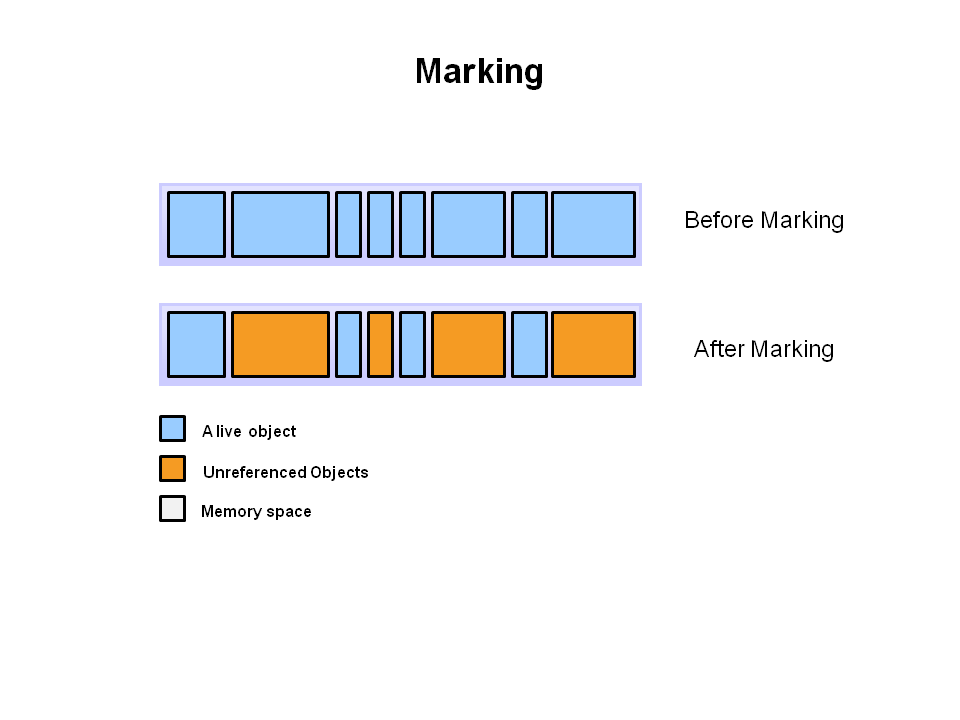
\includegraphics[width=0.9\textwidth]{figures/fundamentals_garbage_collector_marking.PNG}
    \caption[Illustration: Garbage Collector marking memory for deletion \cite{java_garbage_collector}]{Garbage Collector marking memory for deletion}
    \label{fig:gc_mark}
\end{figure}

\begin{figure}[htb]
    \centering
    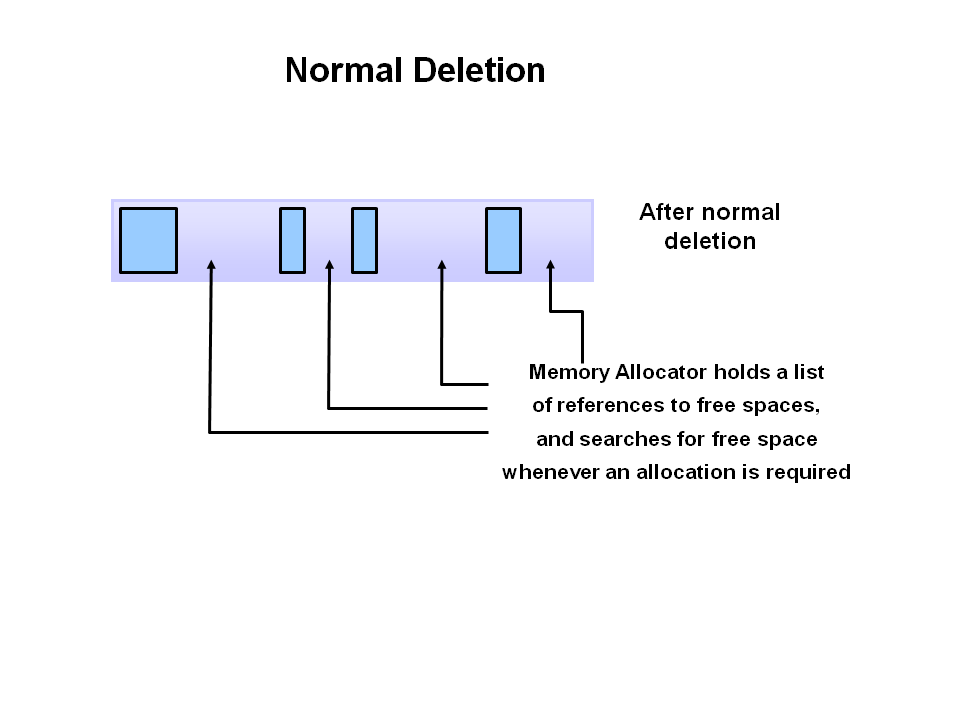
\includegraphics[width=0.9\textwidth]{figures/fundamentals_garbage_collector_deletion.PNG}
    \caption[Illustration: Garbage Collector deleting marked memory \cite{java_garbage_collector}]{Memory layout after deletion of unused pieces of memory}
    \label{fig:gc_delete}
\end{figure}

\begin{figure}[H]
    \centering
    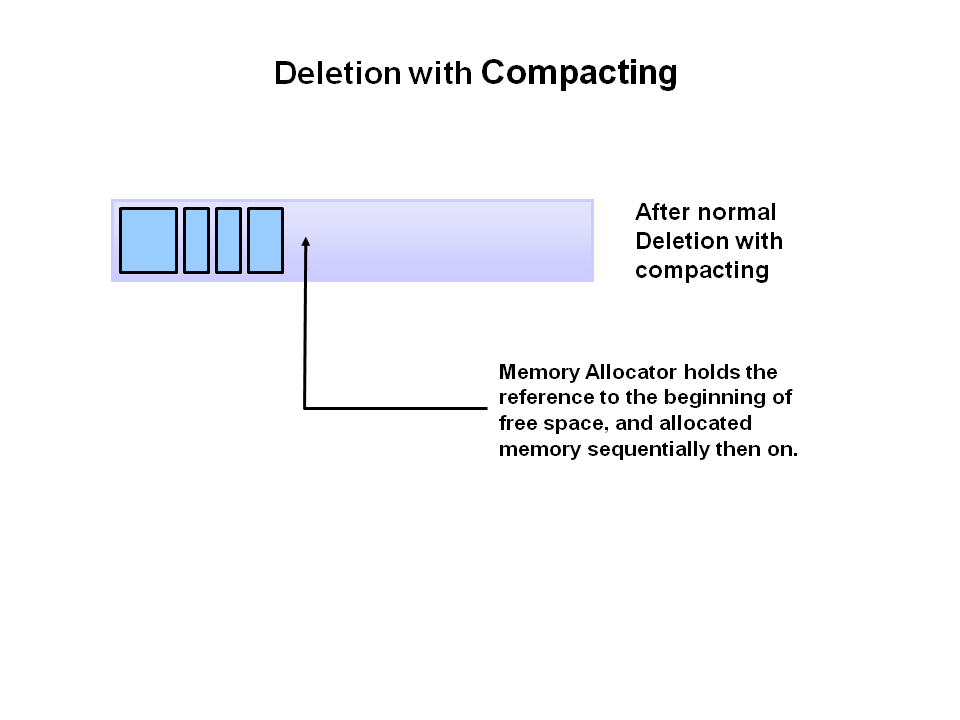
\includegraphics[width=0.9\textwidth]{figures/fundamentals_garbage_collector_compacting.PNG}
    \caption[Illustration: Garbage Collector compacting memory \cite{java_garbage_collector}]{Memory layout after compacting}
    \label{fig:gc_compact}
\end{figure}

Garbage collectors however have a few drawbacks, like unpredictable latency (the running program has to be stopped while the garbage collector is running) and a hit in performance.
The runtime of the programming language, that contains the garbage collector, also needs to be installed on the target system and run alongside the program, using additional
resources which can be problematic in a resource scarce environment like small embedded devices.
Therefore, garbage collected languages are rarely used in embedded systems programming.
Rust uses a different, and unique approach to guarantee memory safety without suffering from any of the aforementioned drawbacks.

\subsubsection{Ownership in Rust}

Rust uses an 'ownership' model \cite{rust_ownership} to make memory safety guarantees at compile time and without the need of a garbage collector,
which is good for safety, and does not negatively impact performance or latency.
This model consists of 3 simple rules:
\begin{enumerate}
    \item Each value has an owner
    \item Each value can only have one owner at a time
    \item When the owner goes out of scope, the value will be dropped
\end{enumerate}

These 'owners' are generally variables. \ref{code:owner} presents a simple example of a 'value' ('\lstinline{5}') and its
'owner' ('\lstinline{owner}').\\

\begin{lstlisting}[style=colorEX,language=Rust,caption={Simple example of a value and it's owner},label={code:owner}]
let owner = 5;
\end{lstlisting}

It doesn't matter that another 'owner' might have the same value. In the code depicted in \ref{code:two_owners}
'\lstinline{owner}' and '\lstinline{owner2}' have the same value, but they are different variables, just like in any
other programming language and have nothing to do with each other. They are different 'owners'.\\

\begin{minipage}{\textwidth}
\begin{lstlisting}[style=colorEX,language=Rust,caption={Simple example of two owners},label={code:two_owners}]
let owner = 5;
let owner2 = 5;
\end{lstlisting}
\end{minipage}


If one variable is assigned to another, one of two things happens; if the value is saved on the stack like in
example \ref{code:copy} the value is simply copied to the second variable, and now '\lstinline{owner}' and '\lstinline{owner2}'
hold the same value, but other than that have nothing to do with each other. They are different 'owners'.\\

\begin{minipage}{\textwidth}
\begin{lstlisting}[style=colorEX,language=Rust,caption={Simple example of a copy},label={code:copy}]
let owner = 5;
let owner2 = owner;
\end{lstlisting}
\end{minipage}

\begin{minipage}{\textwidth}
\begin{lstlisting}[style=colorEX,language=Rust,caption={Simple example of a move},label={code:move}]
let owner = String::from("value");
let owner2 = owner;
\end{lstlisting}
\end{minipage}

If the value is stored on the heap like in example \ref{code:move}, the value is not copied, because that could
be potentially very expensive\footnote{The more technical reason why variables for certain types cannot be copied
is that they do not implement the 'Copy' trait. This trait is only implemented for 'small' types like integers,
characters, and so on. A 'String' could theoretically be very large, while integers are limited to a few bytes at most.
However, one could implement this trait for a given type, and then it would be copied.
But this rarely makes sense for 'larger' values, because then copying is computationally expensive.
So usually the desired behavior is that those values are moved.}.
So only the pointer (memory address), size of the data, and the capacity of the memory block is copied.
But now '\lstinline{value}' has two owners, which violates rule 2.
This rule is important because due to rule 3:
\begin{enumerate}
    \item If both variables go out of scope at the same time, the memory would be freed twice.
    \item If only one goes out of scope, the other holds the address of invalid (freed) memory.
\end{enumerate}
To avoid those things '\lstinline{value}' is considered to be 'moved' to its new owner, the variable '\lstinline{owner2}'.
The original owner ('\lstinline{owner}') is no longer valid.\\
This works similarly for functions, and these 3 rules allow the compiler to check for any mistakes that would lead to
a double free, use-after-free or memory that has forgotten to be freed.
However, there is one more important aspect of memory management in Rust; the borrow operator.
The borrow operator ('\lstinline{&}') \cite{rust_borrow} allows other variables access to a value without changing the owner.
There are two more rules for references and borrowing:
\begin{enumerate}
    \item There can be an any number of immutable references to a value.
    \item There can never be more than one mutable reference to a value.
\end{enumerate}
The code snippet \ref{code:borrow} displays a valid use of rule 1 and code snippet \ref{code:mut_borrow} gives both examples
of what is valid and invalid under rule 2.

\begin{minipage}{\textwidth}
\begin{lstlisting}[style=colorEX,language=Rust,caption={Simple example of an immutable borrow},label={code:borrow}]
let mut owner = 5;
let borrower1 = &owner;
let borrower2 = &owner;
\end{lstlisting}
\end{minipage}

\begin{minipage}{\textwidth}
\begin{lstlisting}[style=colorEX,language=Rust,caption={Simple example of a mutable borrow},label={code:mut_borrow}]
let mut owner = 5;
let borrower = &mut owner;

// These 2 statements are not allowed, as the value as already borrowed as mutable.
// let borrower1 = &owner;
// let borrower2 = &mut owner;
\end{lstlisting}
\end{minipage}

\subsection{Embedded Rust}

Developing software that runs directly on hardware differs slightly from 'normal' software due to the lack of an operating system (OS).
When developing for a microcontroller (MCU) there usually is no OS that supervises and manages programs or facilitates communication with peripherals\footnote
{There are real-time operating systems (RTOSs) that run on MCUs that take care of many of these things,
and several ARM MCUs can and sometimes do run Linux. But that is not relevant to this thesis, since the MCU I'm working on doesn't have an OS running on it.}.
Therefore, embedded Rust programs look a little different from those that would run on a Windows, Linux or Mac computer.
\\
First, since there is no operating system to allocate memory, put the code into the right memory space and start the program.
So the developer has to take care of that when creating the executable, which is why 'special' instructions for the linker are necessary.
For Rust programs these instructions are written into a \emph{memory.x} file.
This file contains information about the memory layout of the hardware that the program will be running on.
An example of such a \emph{memory.x} file is displayed in \ref{code:memory_x}.
The \emph{MEMORY} section defines two sections in memory, 'RAM' and 'LTWO'.
\emph{SECTIONS} maps a label to a continuous block of flash memory that the linker can link data to.
In this case this data is put into the 'LTWO' section created above.
After that, a few aliases are created that either correspond to the 'RAM' section or 'LTWO' section.

\newpage
\begin{minipage}{\textwidth}
\begin{lstlisting}[style=colorEX,caption={Example memory.x file},label={code:memory_x}]
MEMORY
{
  /* NOTE K = KiBi = 1024 bytes */
  RAM : ORIGIN = 0x1C000000, LENGTH = 0x00010000
  LTWO : ORIGIN = 0x1C010000, LENGTH = 0x00072000
}

SECTIONS
{
    .l2_data ORIGIN(LTWO) :
    {
        LONG(0x00072000);
        *(.l2_data);
    } > LTWO
}

REGION_ALIAS("FLASH", RAM);

REGION_ALIAS("REGION_TEXT", FLASH);
REGION_ALIAS("REGION_RODATA", FLASH);
REGION_ALIAS("REGION_DATA", RAM);
REGION_ALIAS("REGION_BSS", RAM);
REGION_ALIAS("REGION_HEAP", RAM);
REGION_ALIAS("REGION_STACK", RAM);

\end{lstlisting}
\end{minipage}


However, there are also quite a few differences in the actual program code.
Usually Rust programs contain a main function that looks like the example in Listing~\ref{code:os_main}.
\begin{minipage}{\textwidth}
\begin{lstlisting}[style=colorEX,language=Rust,caption={Standard main function in Rust},label={code:os_main}]
fn main() {
    // contents of main function
}
\end{lstlisting}
\end{minipage}
This works similar to normal C code where the main function either serves as entry point for the program or will be called by the '\lstinline{_start}' function provided by \emph{glibc} \cite{before_main}.
This '\lstinline{_start}' function initializes the program runtime by setting up things like the stack and writing arguments into memory to name a few.
After initialization, the main function is then called.
This is equal for programs that run with or without an OS.\\
The difference in this startup process occurs before the '\lstinline{_start}' function.
If the program runs on a device with an OS, the OS first does some preparation and initialization for the program to run.
The program environment is configured by, among other things, checking permissions (is the user allowed to run this program),
allocating space on the stack and heap, initializing the stack pointer, linking dynamically linked libraries and calling pre-initialization functions \cite{before_main}.
Once the program environment is configured, the programs '\lstinline{_start}' is called by the OS.


When a program is running on 'bare-metal' (meaning without an OS or even a bootloader that launches the  application), this process is more crude.
The '\lstinline{_start}' function still serves as the entry point for the program, but there are fewer steps involved in getting there.
After the application is compiled by the programmer, it is 'flashed' onto the device, meaning written to flash memory.
When the processor is powered on, it will copy the program into Random Access Memory (RAM) and jump to the reset interrupt vector address.
The programs reset interrupt handler will then initialize the system and configure any necessary hardware components
like registers, external RAM or the Memory Management Unit (MMU).
After that the handler jumps to '\lstinline{_start}' (if present) \cite{before_main}.\\\\
Due to the lack of an OS, there is no cleanup after the program ended either.
As a matter of fact, since the program will be the only thing running on the hardware,
the main function will never return, for our intents and purposes.
The program also only really stops when the device is turned off or reset.

\begin{minipage}{\textwidth}
\begin{lstlisting}[style=colorEX,language=Rust,caption={Example main function for the pulp-platform},label={code:embedded_main}]
#![no_main]

use riscv_rt::entry;

#[entry]
fn main() -> ! {
    // code
    loop {}
}
\end{lstlisting}
\end{minipage}

Listing~\ref{code:embedded_main} displays a main function alike to the ones I've used in my programs.
The '\lstinline{#![no_main]}' directive tells the compiler that I will not use the standard main function.
Since this function will never return, the return type needs to specify exactly that.
In Rust, return types are specified using the '\lstinline{->}', followed by the type \cite{rust_return}.
Replacing the type with a '\lstinline{!}' indicates that the function doesn't return \cite{rust_never_type}.
\\
The '\lstinline{#[entry]}' attribute, imported by the '\lstinline{use riscv_rt::entry}' statement, is used to declare the entry point of the program \cite{riscv_rt_entry}
The requirement for this attribute is that the function never returns, which also why the loop at the end is necessary.
\\\\
This is close to a working program, but not exactly.
Without the OS, the device is also not able to use the standard library.
Which is why the '\lstinline{#![no_std]}' directive is necessary, as it prevents Rust from loading the standard library \cite{rust_no_std}.
However, the standard library provides a lot of useful features, like a dynamic memory allocator or a panic handler.
So these features need to be replaced by their own crates, if available.
The crates that provide those features in this case are called the '\lstinline{pulpissimo_hal}' and '\lstinline{pulpissimo_pac}'.
They act as an abstraction layer over and provide an interface to interact with the hardware.
The Peripheral Access Crate (PAC) provides a code abstraction over the hardware registers and peripherals.
The Hardware Abstraction Layer (HAL) contains drivers that use the PAC to provide a software interface
to interact and control the hardware.
These drivers can then be used to implement programs that do something like light up an LED, display something on a screen,
without necessarily knowing anything out the functionality of the underlying hardware.
These abstractions make it easier to develop a wide array of software because the programmer doesn't have to concern themselves
with things like registers and what bits need to be set to make something work, or the functionality of buses or how to draw
something on a screen.
\\
A minimal example of a running program can be found in Listing~\ref{code:min_example}.
This minimal example doesn't use any features from the '\lstinline{pulpissimo_pac}' directly, which is why it is not 'included'.
Also, the endless loop at the end is replaced by the '\lstinline{exit}' function from the '\lstinline{pulpissimo_hal}' crate.
This only matters if the program is running on simulated hardware. When running the program on real hardware, the '\lstinline{exit}' function is
for all intents and purposes equal to an endless loop \cite[Ch 4.3.10]{rust_pulp}.
This example also uses the '\lstinline{println}' macro from the '\lstinline{pulpissimo_hal}' crate to write messages
to standard-out (stdout), when running in a simulation, or send them using a universal asynchronous receiver-transmitter (UART)
to be viewed in software like minicom, if the program is running on real hardware.

\newpage

\begin{minipage}{\textwidth}
\begin{lstlisting}[style=colorEX,language=Rust,caption={Minimal example of a program running on the pulpissimo hardware},label={code:min_example}]
#![no_main]
#![no_std]

use riscv_rt::entry;
use panic_halt as _;
use pulpissimo_hal::{exit, println};

#[entry]
fn main() -> ! {
    println!("Hello, world!");

    exit(0)
}
\end{lstlisting}
\end{minipage}


\section{Microphone technology}

A microphone consists of a diaphragm and a transducer.
Sound waves cause the diaphragm to vibrate, and
the transducer turns those vibrations into an electrical signal.
This section will introduce one common way to send audio data to different
components of a system as well as methods to encode that analog electrical
signal into a more easily processable, digital representation.

\subsection{I2S}

The inter-IC sound ($I^2S$) \cite{i2s} bus is a serial link that has been developed especially for digital audio.
It uses three lines, one serial data line (SD), which is used to transmit data, one continuous serial clock line (SCK),
which is used as the clock, and one word select line (WS).
$I^2S$ can be used in different configurations, but the master always provides WS and SCK.

\subsubsection{Serial Data}

The data consists of signed integers (in two's complement).
Due to possible differences between the word lengths and neither the transmitter nor the
receiver having any knowledge about the capabilities of the other, the 'most significant bit' (MSB) is transmitted first.
This is the bit with the highest value in a binary number, usually it is the bit in the left-most position,
while the 'least significant bit' (LSB) is located on the right end of the binary sequence.
In the transmission, the MSB has a fixed position, which means that the position of the LSB
is variable due to possible size differences between the word lengths of transmitter and receiver,
and it being dependent on the word length.\\
So when the word length of the system exceeds that of the transmitter, the LSBs are truncated
for the transmission as demonstrated in Figure~\ref{fig:truncation}.
If the receiver receives more bits than its word length, everything after the LSB
of the receiver is ignored, and if the receiver gets fewer bits than its word length,
the missing bits are set to 0.\\
Furthermore, data sent by the transmitter can either be synchronized with a trailing or leading edge
of the clock signal, however received data must be latched onto the leading edge.


\begin{figure}[htb]
    \centering
    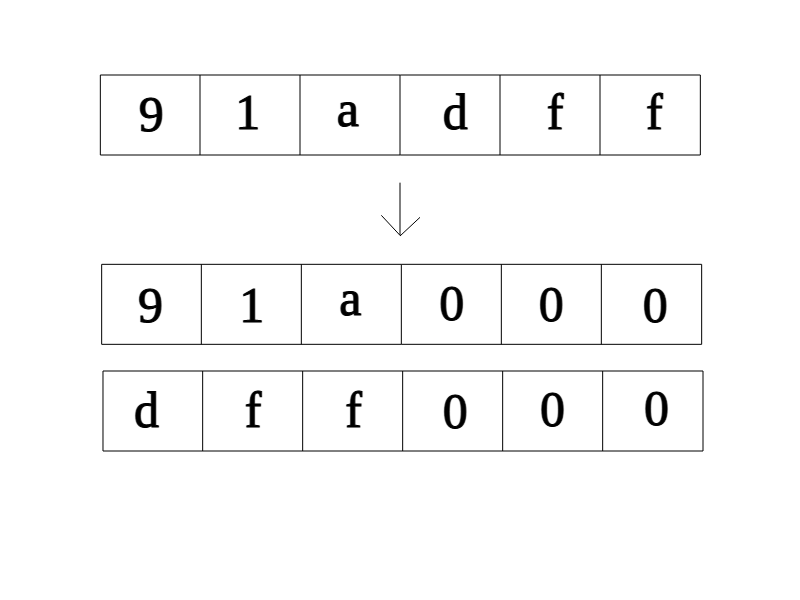
\includegraphics[width=0.9\textwidth]{figures/fundamentals_truncation.png}
    \caption[Illustration: Truncation of words]{Example of a longer word being split into two with the lower bits being set to zero}
    \label{fig:truncation}
\end{figure}

\subsubsection{Word Select}

Word select determines the transmission channel, where 0 means the left channel and 1 means the right one.
It can be changed on a trailing or leading edge of the clock signal and the WS line changes one clock period
before the MSB is transmitted.
For the purpose of what I do in this thesis, WS is not relevant and will be tied to ground unless mentioned otherwise.

\subsection{Pulse Density Modulation}

Pulse Density Modulation (PDM) is one way to represent an analog signal with a binary signal.
The density of high/low signals at a given sampling rate encodes the state of the analog signal.
So the analog signal is encoded using only 1 bit at a high sampling rate.\\
Therefore, a constant bit stream of 1s would represent that the amplitude of the analog signal is maxed out,
while a constant bit stream of 0s would represent that the amplitude of the analog signal is at its lowest value.
Alternating 1s and 0s represent an amplitude of exactly 0.\\\\
While many digital audio systems use Pule Code Modulation (PCM), which, in contrast to PDM, uses multiple bits to represent a signal,
PDM is used a lot in mobile phones \cite{pdm_utexas} due to its simplicity and low cost.
PDM is similar to '1-bit-PCM', however a one bit wide PCM encoded signal would be much too noisy to be useful.
So to counteract the noise increase of only using 1 bit the signal is 'over sampled', thereby increasing the bandwidth of the system.
The new spectrum that is created by oversampling the signal has such a high frequency that it is out of audible range of the human ear.
'Noise Shaping' can then be used to 'push' noise into that new spectrum, thus removing it from the audible signal \cite{pdm_texas}.

\section{Microphones}

This section introduces one PDM and one $I^2S$ (which uses PCM) microphone.
These are the microphones that will be used in this thesis.

\subsection{Adafruit I2S MEMS Microphone}

\subsubsection{Technical Specification}

The $I^2S$ MEMS microphone from Adafruit \cite{i2s_mic} is a digital microphone.
It requires a supply voltage between \SI{1.62}{\volt} and \SI{3.6}{\volt} while drawing a current of \SI{600}{\micro\ampere}.
During sleep mode the current draw is reduced to \SI{10}{\micro\ampere}, and the clock frequency is lowered from anything between
\SI{2048}{\kilo\hertz} and \SI{4096}{\kilo\hertz} to \SI{900}{\kilo\hertz}.
A logical high is read for any voltage between 65\% of the supply voltage ($V_{DD}$) and $V_{DD}$ + \SI{0.3}{\volt},
and a logical low is read for any voltage between \SI{-0.3}{\volt} and 35\% of $V_{DD}$ \cite{i2s_mic_datasheet}.

\subsubsection{Pinout}

The breakout board has 6 pins, $V_{DD}$ and Ground (GND), which are responsible for power, as well as 4 data pins.
The output of the microphone can be read on 'Data Out' (DOUT), the channel (right/left mono audio) can be changed by
changing the voltage of the 'Select' (SEL) pin, which is set to low (left) by default.
The 'bit clock' (BCLK) is the main clock of the device that determines when data is transmitted, and the 'left/right clock' (LRCLK)
controls whether data is transmitted on the left or right channel.
The LRCLK will also be referred to as 'Word Select' (WS) in some instances \cite{i2s_mic_pinout}.

\subsubsection{Timing}

Figure~\ref{fig:i2s_timing} shows the timing diagram of the $I^2S$ microphone.
A clock period should take between \SI{244.14}{\nano\second} and \SI{488.28}{\nano\second}.
A high or low pulse on the clock should be 35\% of the duration of a period.
The maximum delay of the data from a rising edge of the clock should be \SI{65.92}{\nano\second}
and the clock should take no longer than \SI{3.75}{\nano\second} to rise from low to high \cite{i2s_mic_datasheet}.
\\
WS has to change on a falling edge of the clock (BCLK in this case).
Data is sent with the MSB first and delayed by one clock cycle after a change in WS.

\begin{figure}[htb]
    \centering
    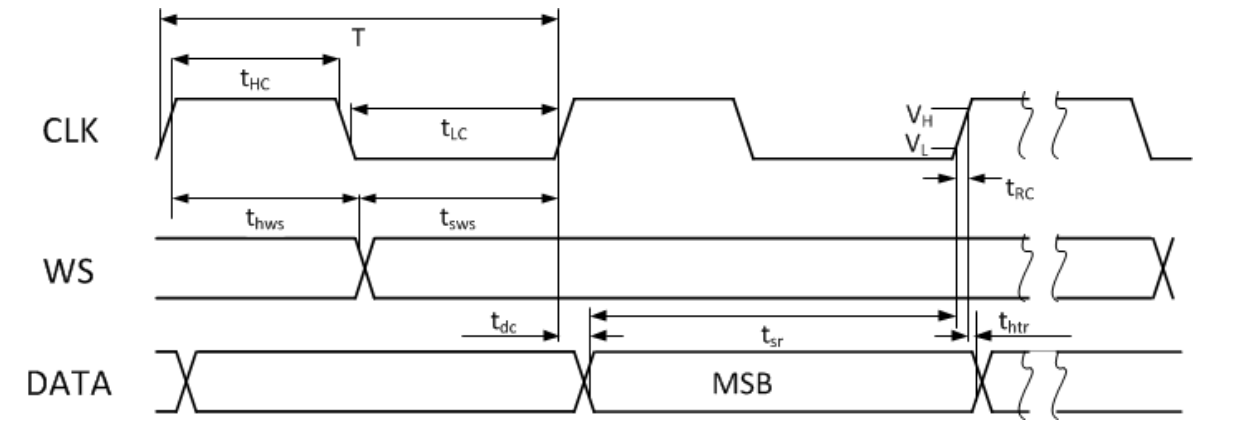
\includegraphics[width=0.9\textwidth]{figures/i2s_timing.png}
    \caption[Timing diagram of the SPH0645LM4H-B $I^2S$ mic \cite{i2s_mic_datasheet}]{Timing diagram of the $I^2S$ microphone}
    \label{fig:i2s_timing}
\end{figure}

\subsection{Adafruit PDM MEMS Microphone}

\subsubsection{Technical Specification}

The PDM MEMS microphone from Adafruit \cite{pdm_mic} is a digital microphone.
It uses the $I^2S$ bus to communicate, but instead of the typical 24 bit encoding of $I^2S$ microphones, PDM microphones only use 1 bit.
It requires a supply voltage between \SI{1.64}{\volt} and \SI{3.6}{\volt} while drawing a current of \SI{600}{\micro\ampere}, with a clock
frequency from \SI{1}{\mega\hertz} to \SI{3.25}{\mega\hertz}.
However, the clock frequency should be reduced to a maximum of \SI{0.23}{\mega\hertz} while the microphone is in 'power-down' mode.
During power down mode the current draw is reduced to \SI{20}{\micro\ampere}.
A logical high is read for any voltage between 65\% of ($V_{DD}$) and $V_{DD}$ + \SI{0.3}{\volt},
and a logical low is read for any voltage between \SI{-0.3}{\volt} and 35\% of $V_{DD}$ \cite{pdm_mic_datasheet}.

\subsubsection{Pinout}

The breakout board of the PDM microphone, in contrast to the breakout board of the $I^2S$ microphone, only has 5 pins.
$V_{DD}$ and Ground (GND), serve the same purpose, but it only needs 3 data pins.
The output of the PDM microphone can be read on 'PDM Data Out' (DAT), and the PDM microphone also has a SEL pin (also referred to as L/R in the timing diagram),
which works the same way as it does in the $I^2S$ microphone.
However, it only has one clock line (CLK), and no WS \cite{pdm_mic_pinout}.

\subsubsection{Timing}

Figure~\ref{fig:pdm_timing} shows the timing diagram for the PDM microphone.
Based on the clock frequency, a period in normal mode should take between \SI{308}{\nano\second} and \SI{1000}{\nano\second}.
The right channel (PDM R) is latched onto the rising edge of the clock and is enabled if the L/R pin is set accordingly.
It is disabled on the falling edge of the clock.
The left channel (PDM L) is latched onto and thus enabled on a falling edge of the clock (assuming L/R is set accordingly),
and disabled on a rising edge.
According to data acquired from design simulations by manufacturer,
PDM L and PDM R takes at least \SI{18}{\nano\second}, while disabling PDM L and PDM R takes at most \SI{16}{\nano\second}.


\begin{figure}[htb]
    \centering
    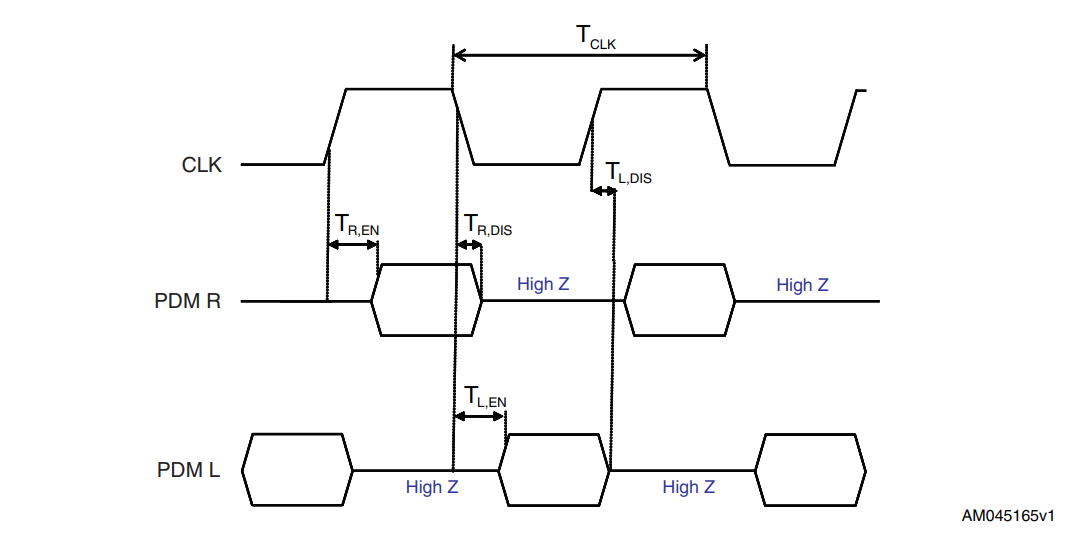
\includegraphics[width=0.9\textwidth]{figures/pdm_timing.png}
    \caption[Timing diagram of the MP34DT01-M PDM MEMS mic \cite{pdm_mic_datasheet}]{Timing diagram of the PDM MEMS microphone}
    \label{fig:pdm_timing}
\end{figure}

\cleardoublepage

\ifthenelse{\boolean{english}}
	{\chapter{Related Work}}
	{\chapter{Stand der Technik}}
\label{cha:related_work}
% =============================================================================
% FILE NAME : 02_related_work.tex
% DEPARTMENT: University of Tuebingen
% AUTOR     : Tom Schammo
% =============================================================================
% CONTENT   : Include for chapter "Related Work"
% =============================================================================

\section{Rust on the PULPissimo}

The code in this thesis is built upon the foundations built by Raphael Vogelgsang in his thesis \emph{'Rust auf der RISCV Plattform PULPissimo – Entwicklung und
Evaluation'} \cite{rust_pulp}.
He built the Peripheral Access Crate (PAC) and Hardware Abstraction Layer (HAL) which I use and extend to add support for the UltraTrail architecture.
The PAC provides direct access to peripherals and has been generated using the '\lstinline{svd2rust}' tool \cite{svd2rust}.
This tool uses a System View Description (SVD) file, which uses the XML format to describe certain properties like registers and peripherals, and are
thereby unique for each microcontroller.
SVD files are usually provided by the vendor, but in this case it had to be written from scratch.
The HAL builds upon the PAC and provides a layer of abstraction between the programmer and the hardware.
It implements a user-friendly API that removes the need for detailed knowledge about the hardware architecture.

\section{Previous work on the PULPissimo}

The chair for embedded systems has developed some C libraries for the PULPissimo that provide drivers and tests.
They serve as an orientation and comparison for the Rust libraries.

\section{UltraTrail}

UltraTrail is a 'configurable ultra-low power TC-ResNet AI accelerator for efficient keyword spotting' \cite{ultratrail}.
It uses temporal convolutional networks (TCNs) combined with residual networks (TC-ResNet) for intelligent sensor signal processing.
They show superior behavior compared to conventional convolutional neural networks (CNNs) and long short-term memory (LSTM) networks,
which is a type of Recurrent Neural Network (RNN), and commonly used speech recognition applications like keyword spotting or text to speech engines.
TCNs specifically not only appear to be more accurate, but also simpler and clearer compared to LSTMs and GRUs \cite[Ch I]{ultratrail}.\\
UltraTrail uses a variety of units, arrays and layers to provide efficient mapping of the TC-ResNet without sacrificing too much flexibility.
It can execute networks with up to 16 convolutional layers that can be extended with batch normalization (also referred to as CONV-EXT layers),
and uses 6 bit weights and 8 bit feature inputs.\\
The network model is saved in the weight memory (WMEM) and bias memory (BMEM), that
have a capacity of 64 kB and 512 Bytes respectively.
UltraTrail is also equipped with three feature map memories (FMEM) to store input and output
feature maps.
These five memories, surround the 8x8 MAC array with local memory (LMEM) and the Output Processing Uni (OPU) as displayed in figure \ref{fig:ultratrail_arch}.
\\\\
The MAC array is the primary processing unit and enables convolutional computation.
It contains 64 MAC units that are arranged in an 8x8 grid that use the LMEM to store partial sums during computation.
The size of the array allows for almost optimal utilization of the available processing units.
\\
The OPU receives the output features generated by the MAC array and combines bias, ReLU activation,
average pooling and condition computing to complete the remaining post-processing steps.
The results are written back to FMEM.
\\
UltraTrail additionally has a programmable control unit that contains a 672 bit
configuration register, which is big enough so that the network structure
can be described layer by layer.


\begin{figure}[htb]
    \centering
    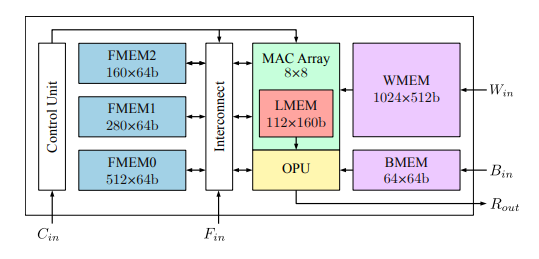
\includegraphics[width=0.9\textwidth]{figures/ultratrail.png}
    \caption[Illustration: The UltraTrail system architecture (Fig. 5)\cite{ultratrail}]{The UltraTrail system architecture}
    \label{fig:ultratrail_arch}
\end{figure}

\section{Keyword spotting in the Industry}

\subsection{Voice Assistants}

Keyword spotting is mainly used in voice assistants (VAs), like Siri by Apple \cite{siri} or Amazon's Alexa \cite{alexa}.
The devices they run on (like Amazon Echo Dot) use keyword spotting to 'activate', after which they start
to 'actively listen' to perform your command.
There are also open source alternatives to the popular products by the aforementioned tech giants, like Mycroft by \lstinline{mycroft.ai} \cite{mycroft}.
Snips.ai used to be another alternative VA to the products by Apple and Amazon, however, they have been acquired by Sonos in November 2019 \cite{sonos_snips}.
Snips used also used a keyword spotting to 'activate' the VA that the user could then communicate with, however, they also advertise their focus
on privacy and offline, on device speech processing.
However, their product was not open source, so there is limited knowledge available about their system.
They do advertise customizable 'wake words', and mentioned hardware requirement on a snapshot of their website \cite{snips_flow}.
It was possible to run their system on devices like the Raspberry Pi 3 \cite{rpi3} or Jetson TX2 \cite{jetson_tx2},
as well as the Snapdragon 410 \cite{snapdragon_410} by Qualcomm, which had been used in phones like the Samsung Galaxy J5 or Xiaomi Redmi 2.
Since there is not a lot of public knowledge available for proprietary systems like Siri, Alexa or Snips, I will take a more in depth look at Mycroft only.

\subsubsection{Mycroft}

Mycroft is an open source \cite{mycroft_gh} and privacy focused VA \cite{mycroft}.
It runs a variety of devices like the Raspberry Pi, common desktop devices, but also custom hardware, the manufacturer claims.
Like Alexa, Mycroft can be extended by adding skills \cite{mycroft_skills}, which can either be acquired for free on their marketplace,
from GitHub or self-made.\\\\
Mycroft consists of several technologies; 'Mimic' \cite{mycroft_mimic3}, their text-to-speech engine, 'Adapt' \cite{mycroft_adapt} and 'Padatious' \cite{mycroft_padatious},
their intent parsers for natural language understanding, and most interestingly for this thesis, 'Precise' \cite{mycroft_precise} their wake word listener.\\
Precise uses a type of RNN, a Grated Recurrent Unit (GRU), illustrated in \ref{fig:precise_gru}.


\begin{figure}[htb]
    \centering
    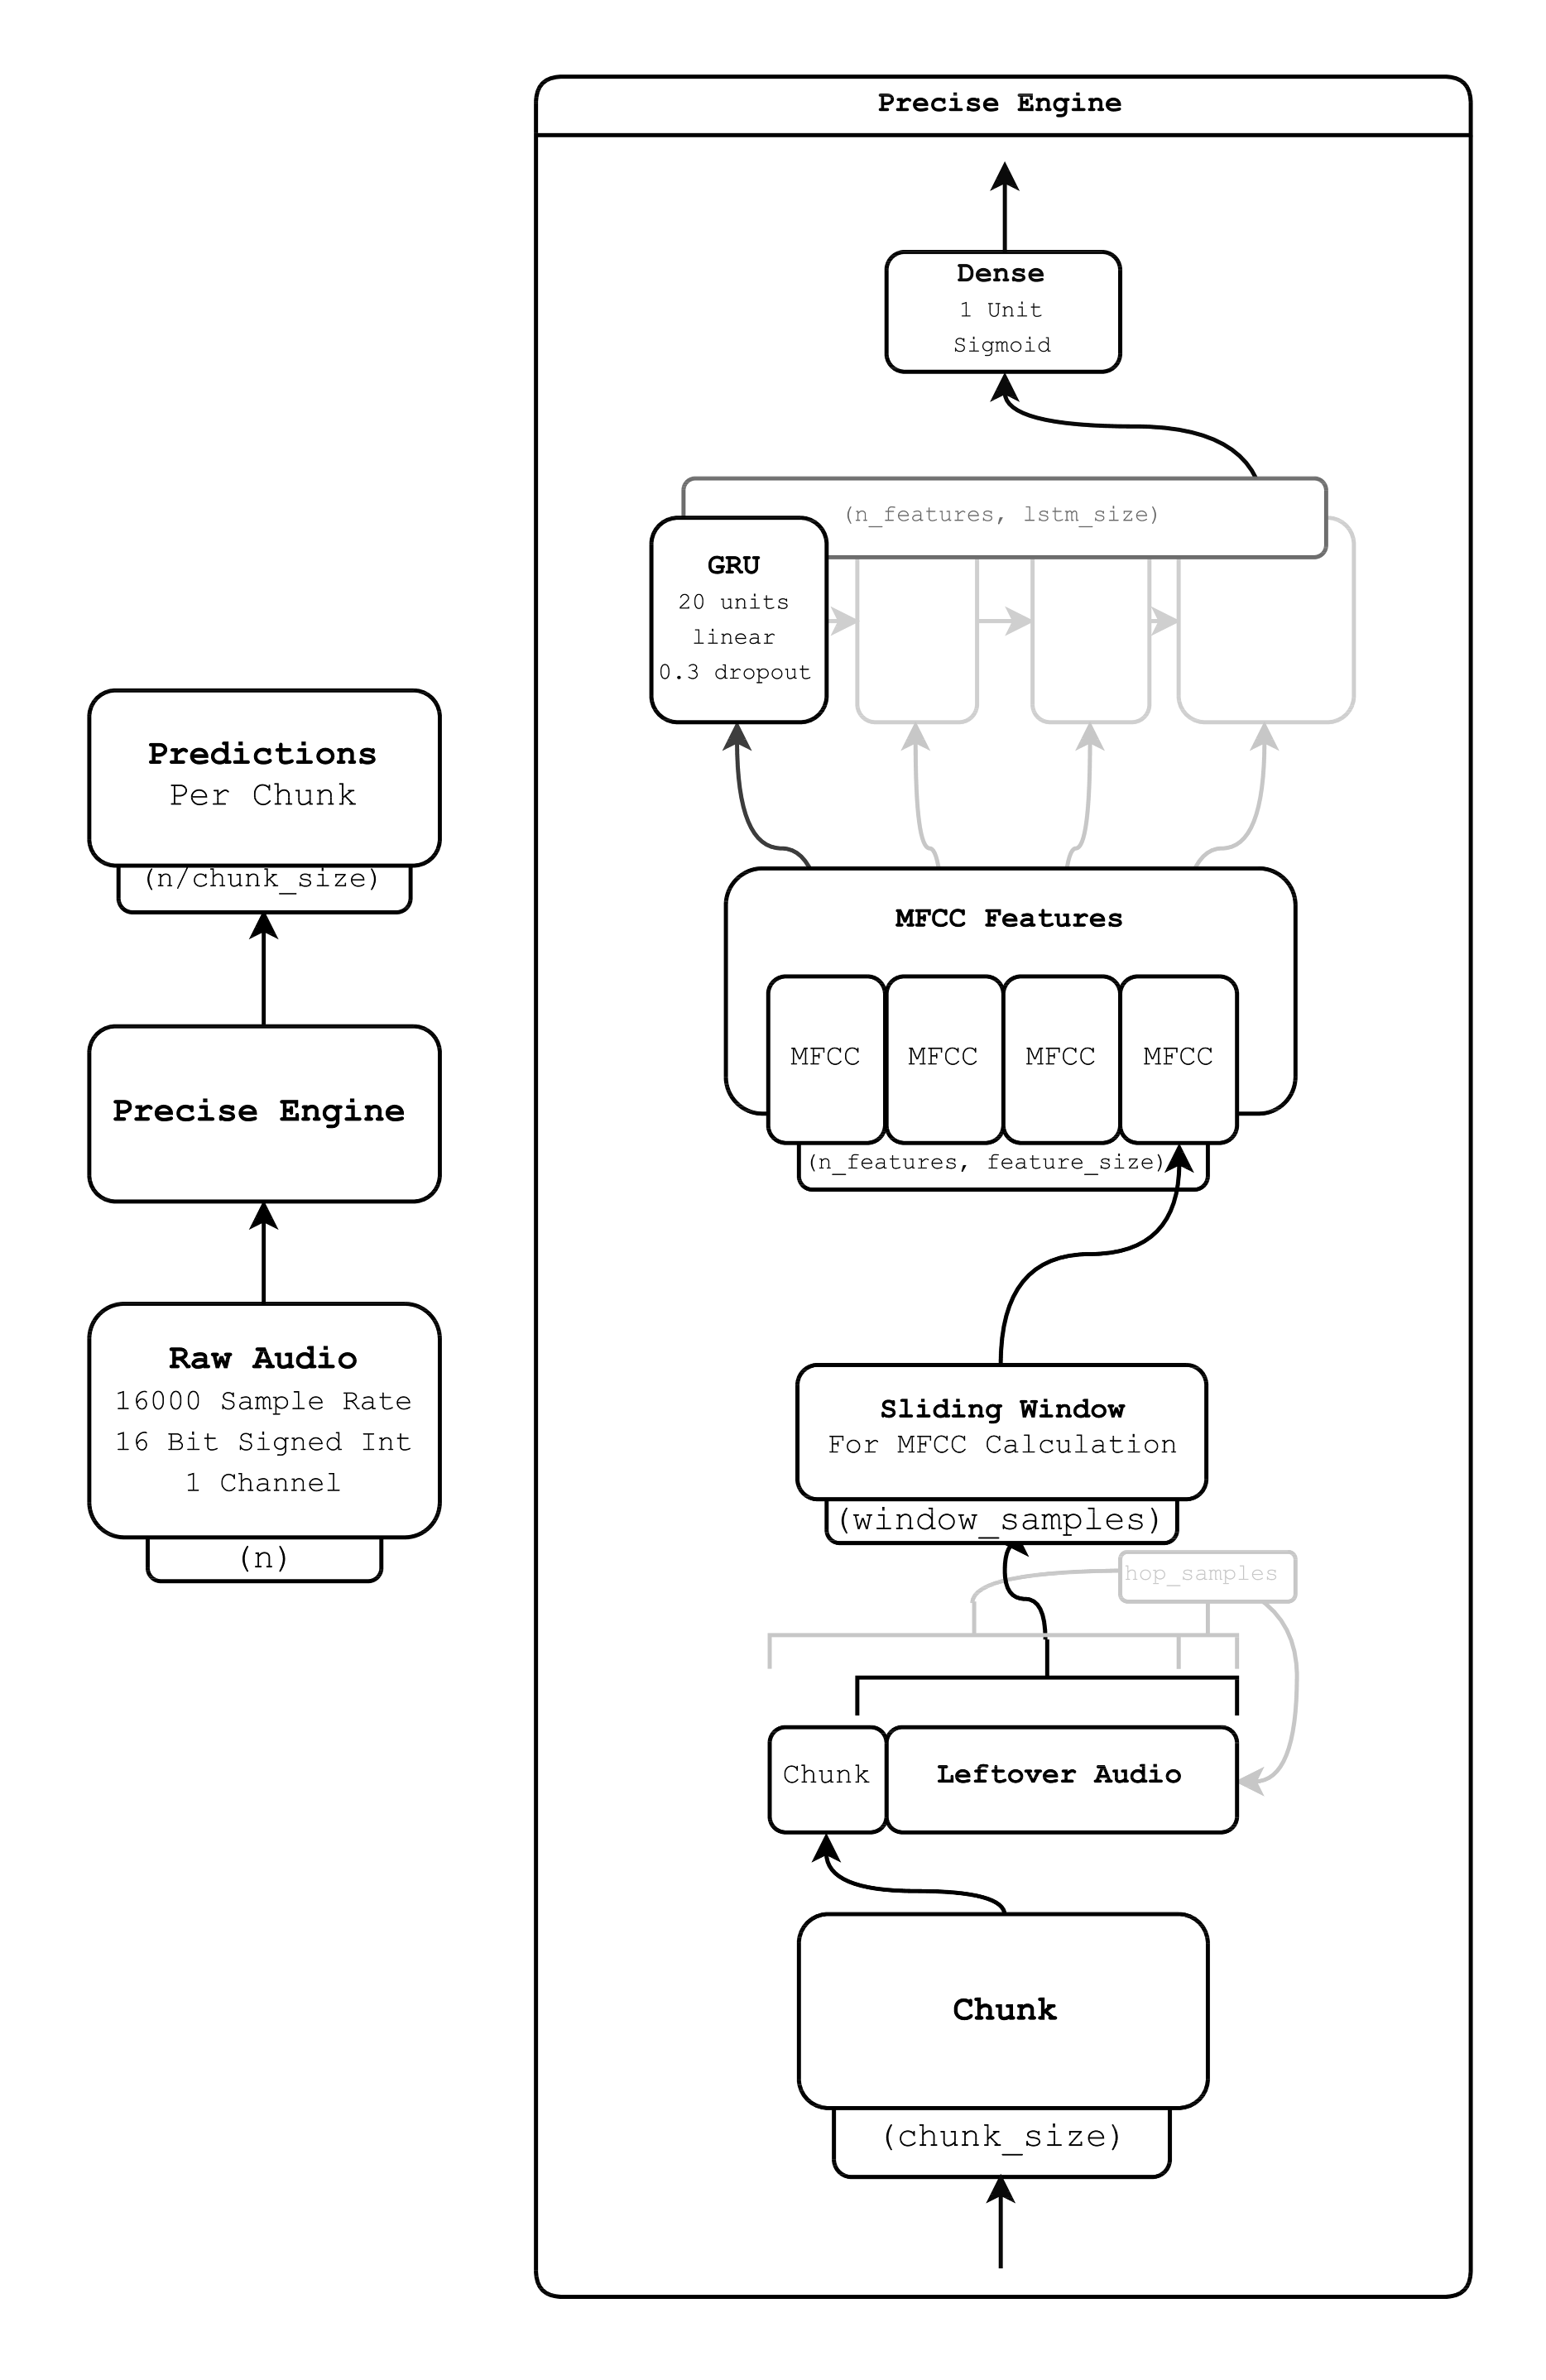
\includegraphics[width=0.9\textwidth]{figures/precise_engine.PNG}
    \caption[Illustration: The 'Precise' engine \cite{mycroft_precise}]{The 'Precise' engine illustrated}
    \label{fig:precise_gru}
\end{figure}



\cleardoublepage

\ifthenelse{\boolean{english}}
	{\chapter{Concept}}
	{\chapter{Konzept}}
\label{cha:concept}
% =============================================================================
% FILE NAME : 03_concept.tex
% DEPARTMENT: University of Tuebingen
% AUTOR     : Paul Palomero Bernardo & Konstantin Lübeck
% =============================================================================
% CONTENT   : Include for chapter "Concept"
% =============================================================================
Mit das Wichtigste natürlich!

Hier wird der eigene Ansatz vorgestellt. Der Titel sollte natürlich nicht einfach Konzept heißen, sondern konkret den eigenen Ansatz benennen.

% TODO Idee der arbeit

% NOTE:
%
% - Rust immer mehr popularity
% - Aber neu, also Lücken
% - Rust eco system auf der pulp-platform
% - Raphaels arbeit
% - UltraTrail und embedded AI
% - Resultate (I2S und PDM, UltraTrail)

\cleardoublepage

\ifthenelse{\boolean{english}}
	{\chapter{Results and Discussion}}
	{\chapter{Ereignisses und Diskussion}}
\label{cha:results_and_discussion}
% =============================================================================
% FILE NAME : results_and_discussion.tex
% DEPARTMENT: University of Tuebingen
% AUTOR     : Tom Schammo
% =============================================================================
% CONTENT   : Include for chapter "Results and Discussion"
% =============================================================================


\section{Microphones}

\subsection{Implementation}

Driver support for $I^2S$ and PDM has already been implemented into the PULPissimo HAL \cite[Cha 4.3.7]{rust_pulp},
however, the microphones, unfortunately, did not work right away for several reasons.
In contrast to the PDM microphone, the $I^2S$ microphone does not work on the PULPissimo chip, due to a hardware compatibility issue.
The $I^2S$ microphone sends a total of 24 bits, a word 18-bit word, and 6 zero bits. But the PULPissimo can only handle 16 bits.
While the PDM microphone is compatible with the PULPissimo chip, the Rust drivers were not mature enough for it to work using Rust.

\subsection{Experiments}

To test the functionality of the microphones I played a \SI{1}{\kilo\hertz} sine wave\footnote{Sine wave audio: \url{https://www.youtube.com/watch?v=3FBijeNg_Gs}},
which I then recorded using the microphone.

\subsubsection{I2S Microphone}

\begin{figure}[H]
    \centering
    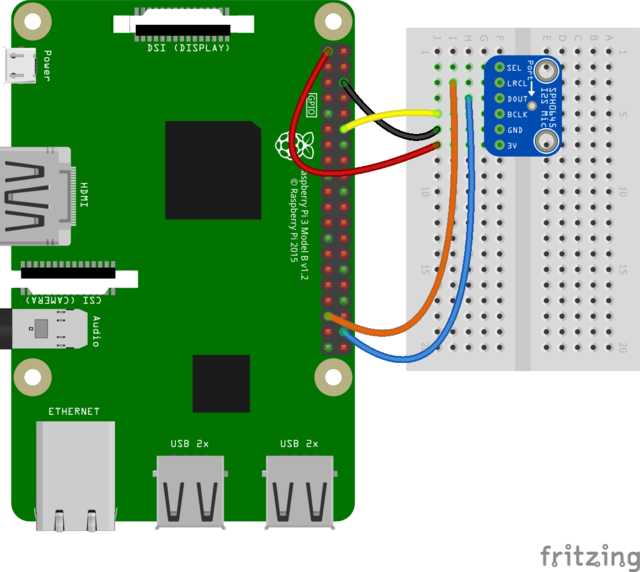
\includegraphics[width=0.5\textwidth]{figures/i2s/wiring_pi.png}
    \caption[$I^2S$ microphone wiring diagram with Raspberry Pi \cite{i2s_wiring}]{$I^2S$ microphone wiring diagram with Raspberry Pi}
    \label{fig:i2s_wiring}
\end{figure}

The $I^2S$ microphone has been wired as displayed in Figure~\ref{fig:i2s_wiring} \cite{i2s_wiring}.
Additionally, SEL has been tied to ground.
The recording was made using this command \lstinline{arecord -D dmic_sv -c2 -r 48000 -f S32_LE -t wav -V mono -v <file name>},
where \emph{<file name>} is the name of the output file.
This creates a 32-bit, PCM-encoded mono WAVE audio file with a sample rate of \SI{48000}{\hertz}.
The \SI{1}{\kilo\hertz} sine wave audio has been played using the speakers of a Redmi Note 7 phone.

\begin{figure}[H]
    \centering
    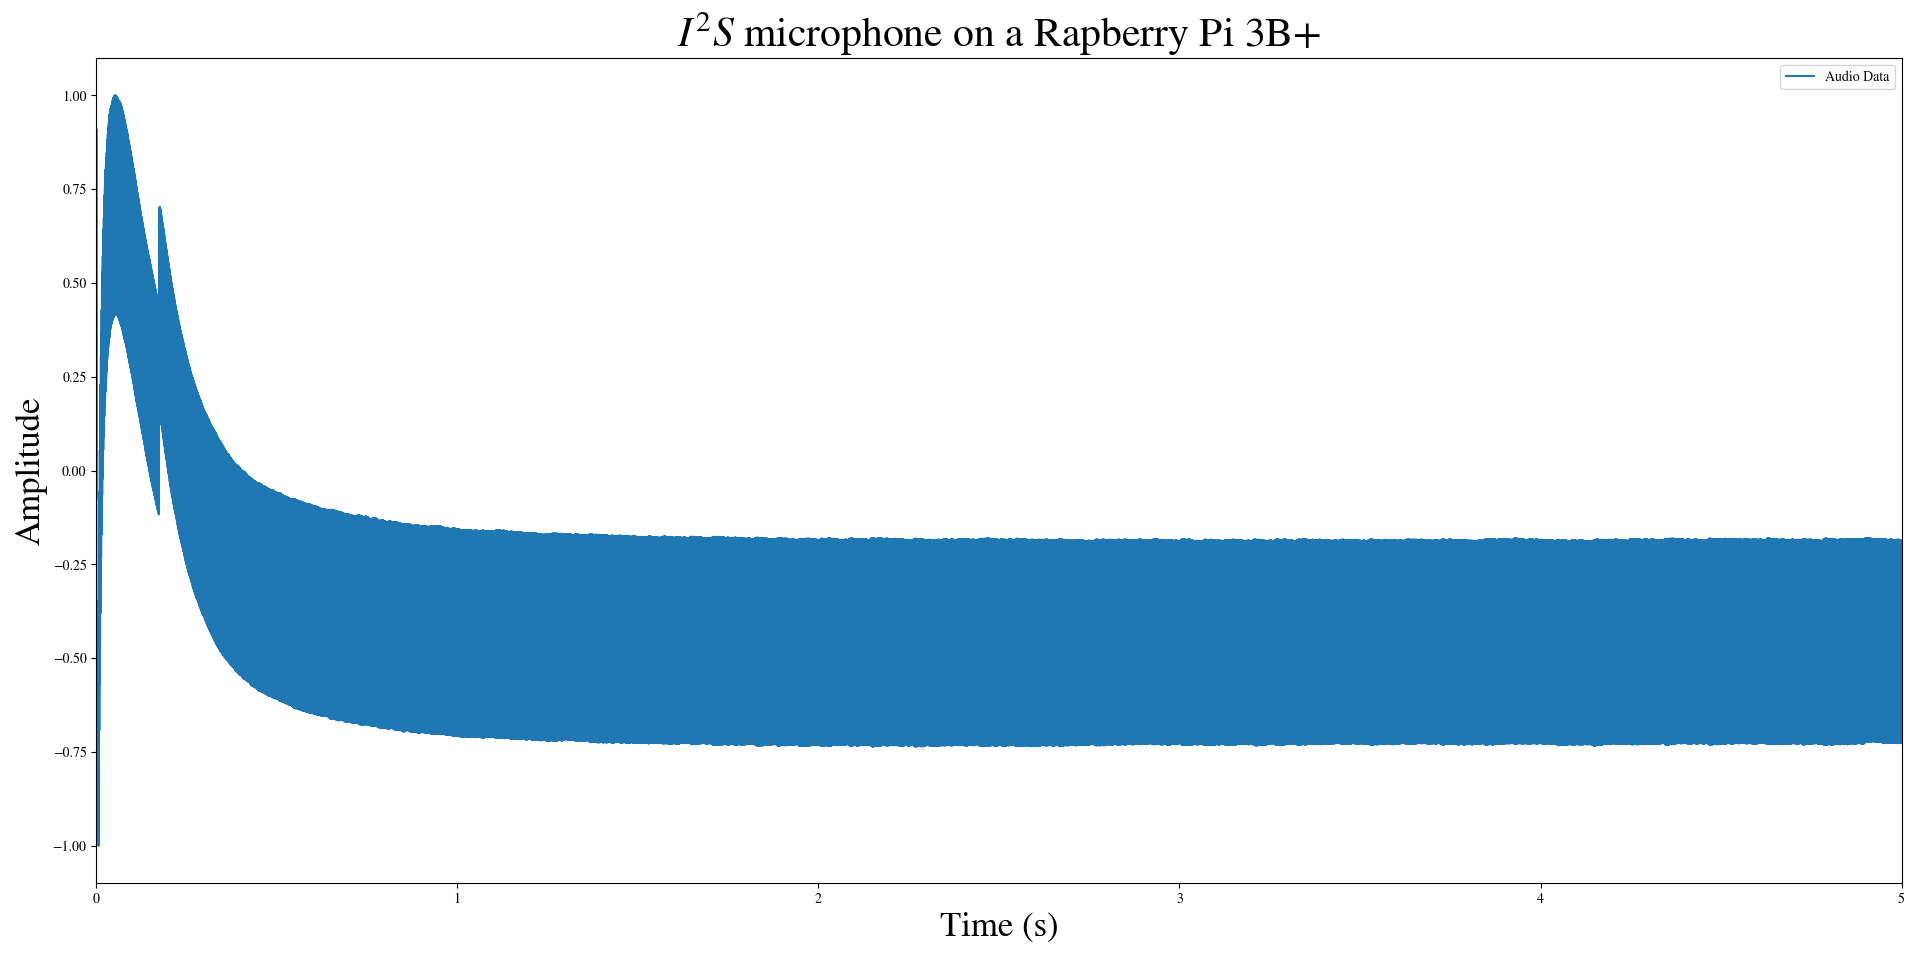
\includegraphics[width=0.9\textwidth]{figures/i2s/i2s_raw_data.png}
    \caption[PCM data of the $I^2S$ microphone plotted]{PCM data of the $I^2S$ microphone plotted}
    \label{fig:i2s_raw}
\end{figure}

When analyzing the raw data displayed in Figure~\ref{fig:i2s_raw}, the spike from seconds 0 to about 0.5
is very noticeable. That is because the microphone seems to have a 'warm-up time', it takes about 1 second for it to be operational and produce clean data.
This has also been noticed on the PULPissimo board with the PDM microphone.
However, after that period, the $I^2S$ microphone is completely operational.
A segment of the recording (normalized) is shown in Figure~\ref{fig:i2s_section}, revealing a clean sine wave.

\begin{figure}[H]
    \centering
    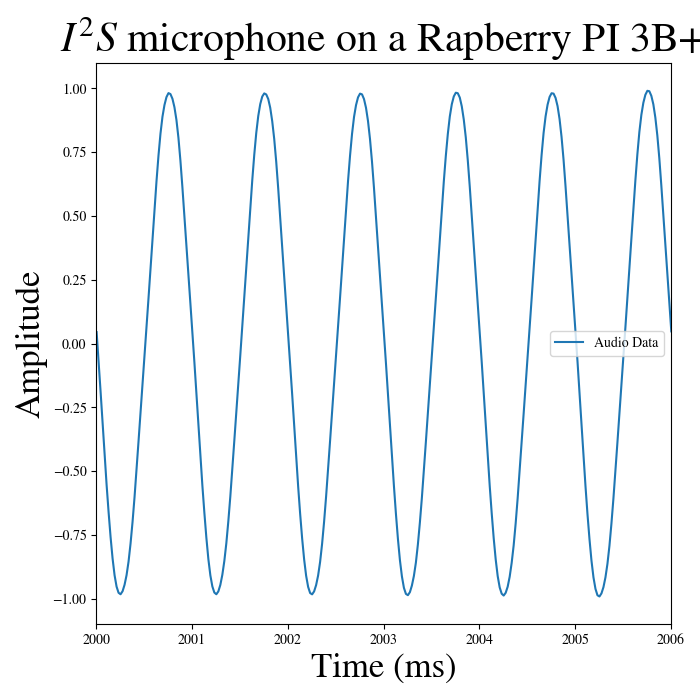
\includegraphics[width=0.9\textwidth]{figures/i2s/i2s_data_recording.png}
    \caption[Sample of normalized PCM data from $I^2S$ microphone]{Sample of normalized PCM data from $I^2S$ microphone}
    \label{fig:i2s_section}
\end{figure}

When taking a close look at a single period and overlaying the data with a perfect sine wave of the same
frequency, displayed in Figure~\ref{fig:i2s_period}, there is a slight, but noticeable discrepancy between the perfect sine
wave and the audio data.
This could have a variety of reasons.
Firstly, the audio that has been played might not have been a perfect sine wave to begin with.
There could've also been variations due to the speakers that had been used, the speakers
might not have produced a 100\% accurate tone.
Or this discrepancy could also be caused by something on the recording side.
Perhaps it is a result of microphone limitations.

\begin{figure}[H]
    \centering
    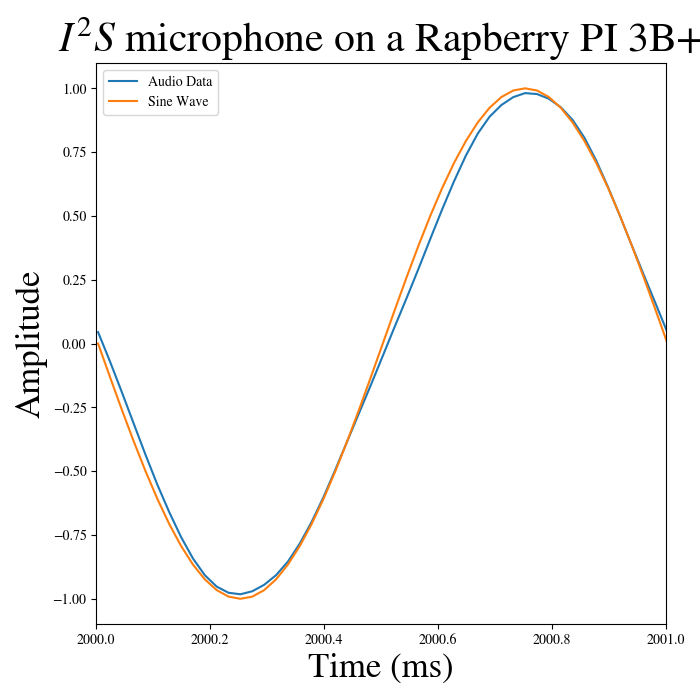
\includegraphics[width=0.9\textwidth]{figures/i2s/i2s_one_period.png}
    \caption[A single period of the normalized audio data, overlaid with a perfect sine wave of the same frequency]{Single period of the audio data, overlaid with sine wave}
    \label{fig:i2s_period}
\end{figure}

\subsubsection{PDM Microphone}

The PDM microphone has been wired as displayed in Figure~\ref{fig:pdm_wiring}.
A logic level converter\footnote{\url{https://cdn-shop.adafruit.com/datasheets/txb0108.pdf}}
has been used because the microphone needs a supply voltage of \SI{3.3}{\volt}, but the
PULPissimo clock uses \SI{1.8}{\volt}.

\begin{figure}[H]
    \centering
    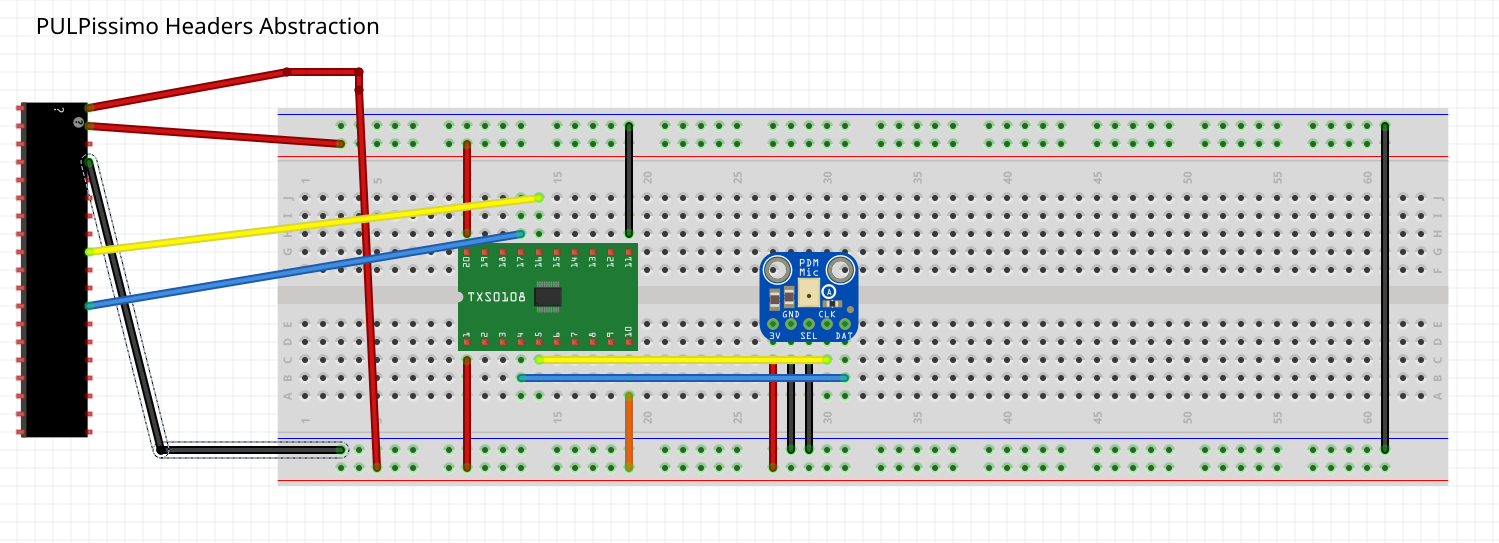
\includegraphics[width=0.9\textwidth]{figures/pdm/wiring.png}
    \caption[PDM microphone wiring with an abstraction for the PULPissimo]{PDM microphone wiring}
    \label{fig:pdm_wiring}
\end{figure}


\begin{figure}[H]
    \centering
    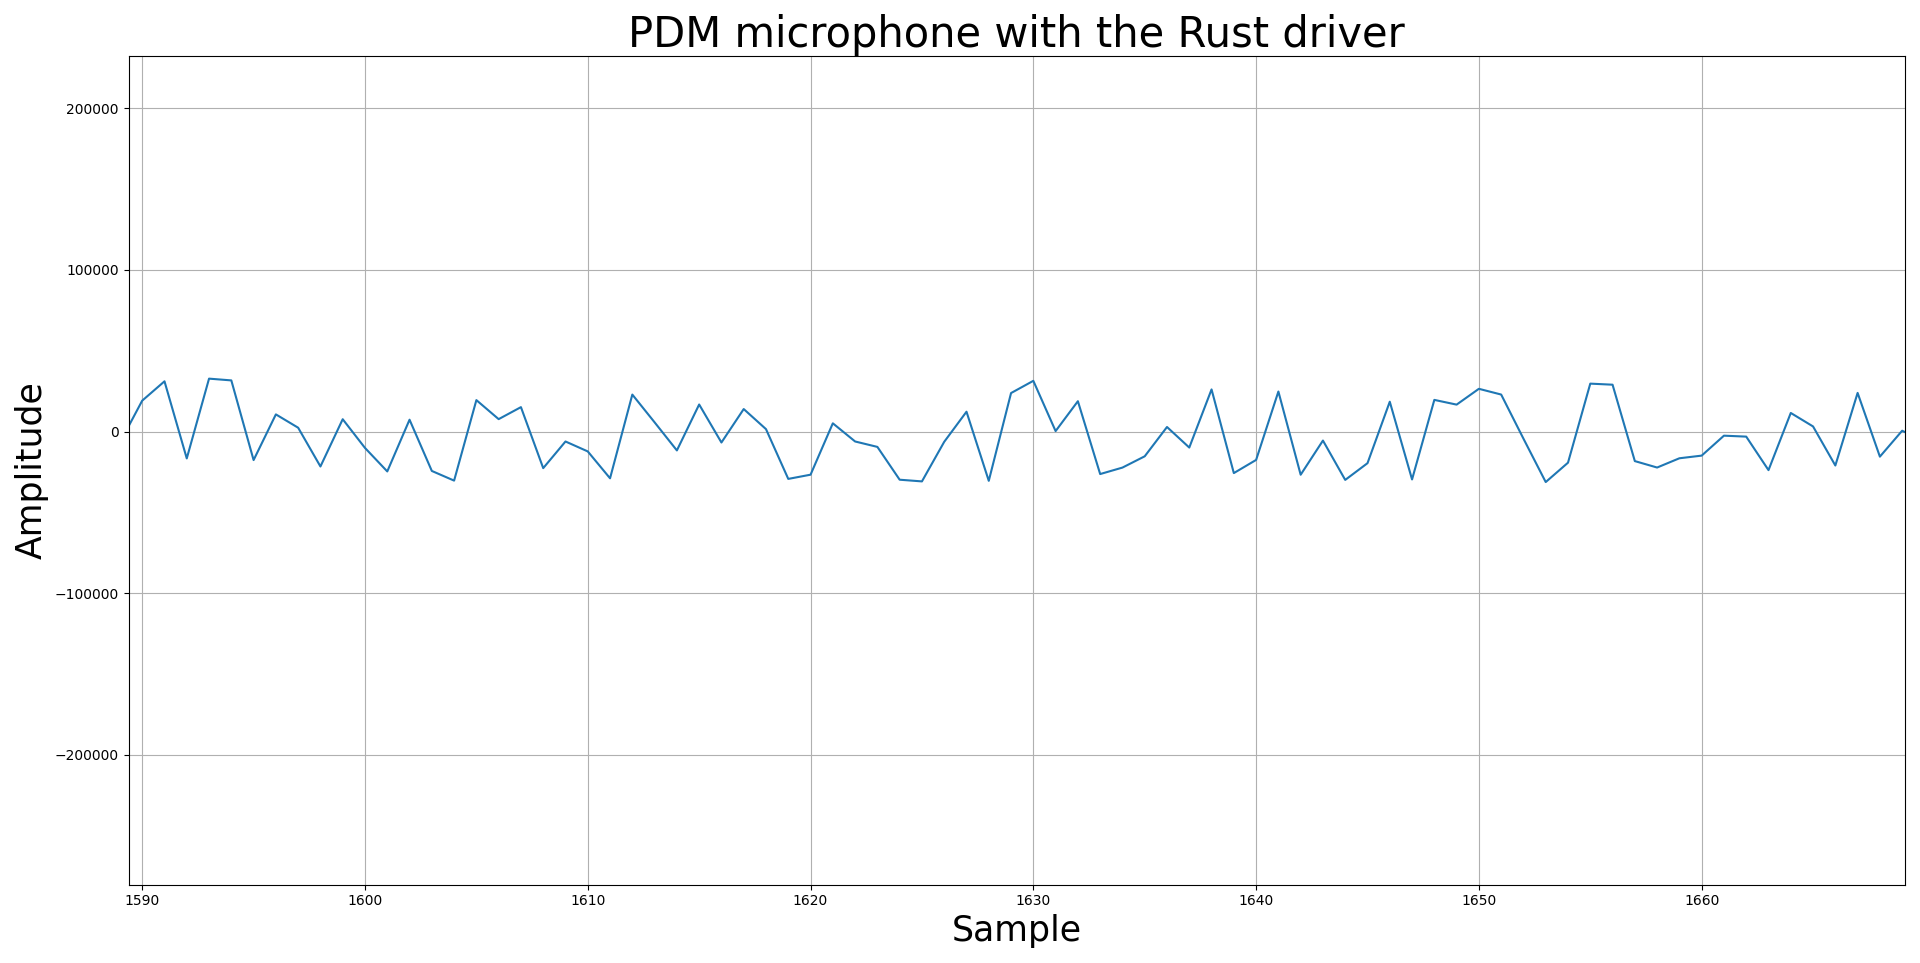
\includegraphics[width=0.9\textwidth]{figures/pdm/pdm_rust.png}
    \caption[Segment of the audio data recorded by the PDM microphone using the Rust driver]{Segment of the audio data recorded by the PDM microphone using the Rust driver}
    \label{fig:pdm_rust}
\end{figure}

Figure~\ref{fig:pdm_rust} shows a section of the recorded PDM data in a PCM encoding, and it is very clear that the driver does not work as intended.
Expected was a sine wave, like in Figure~\ref{fig:pdm_c}, which has been recorded with the same microphone, same wiring using the C driver.

\begin{figure}[H]
    \centering
    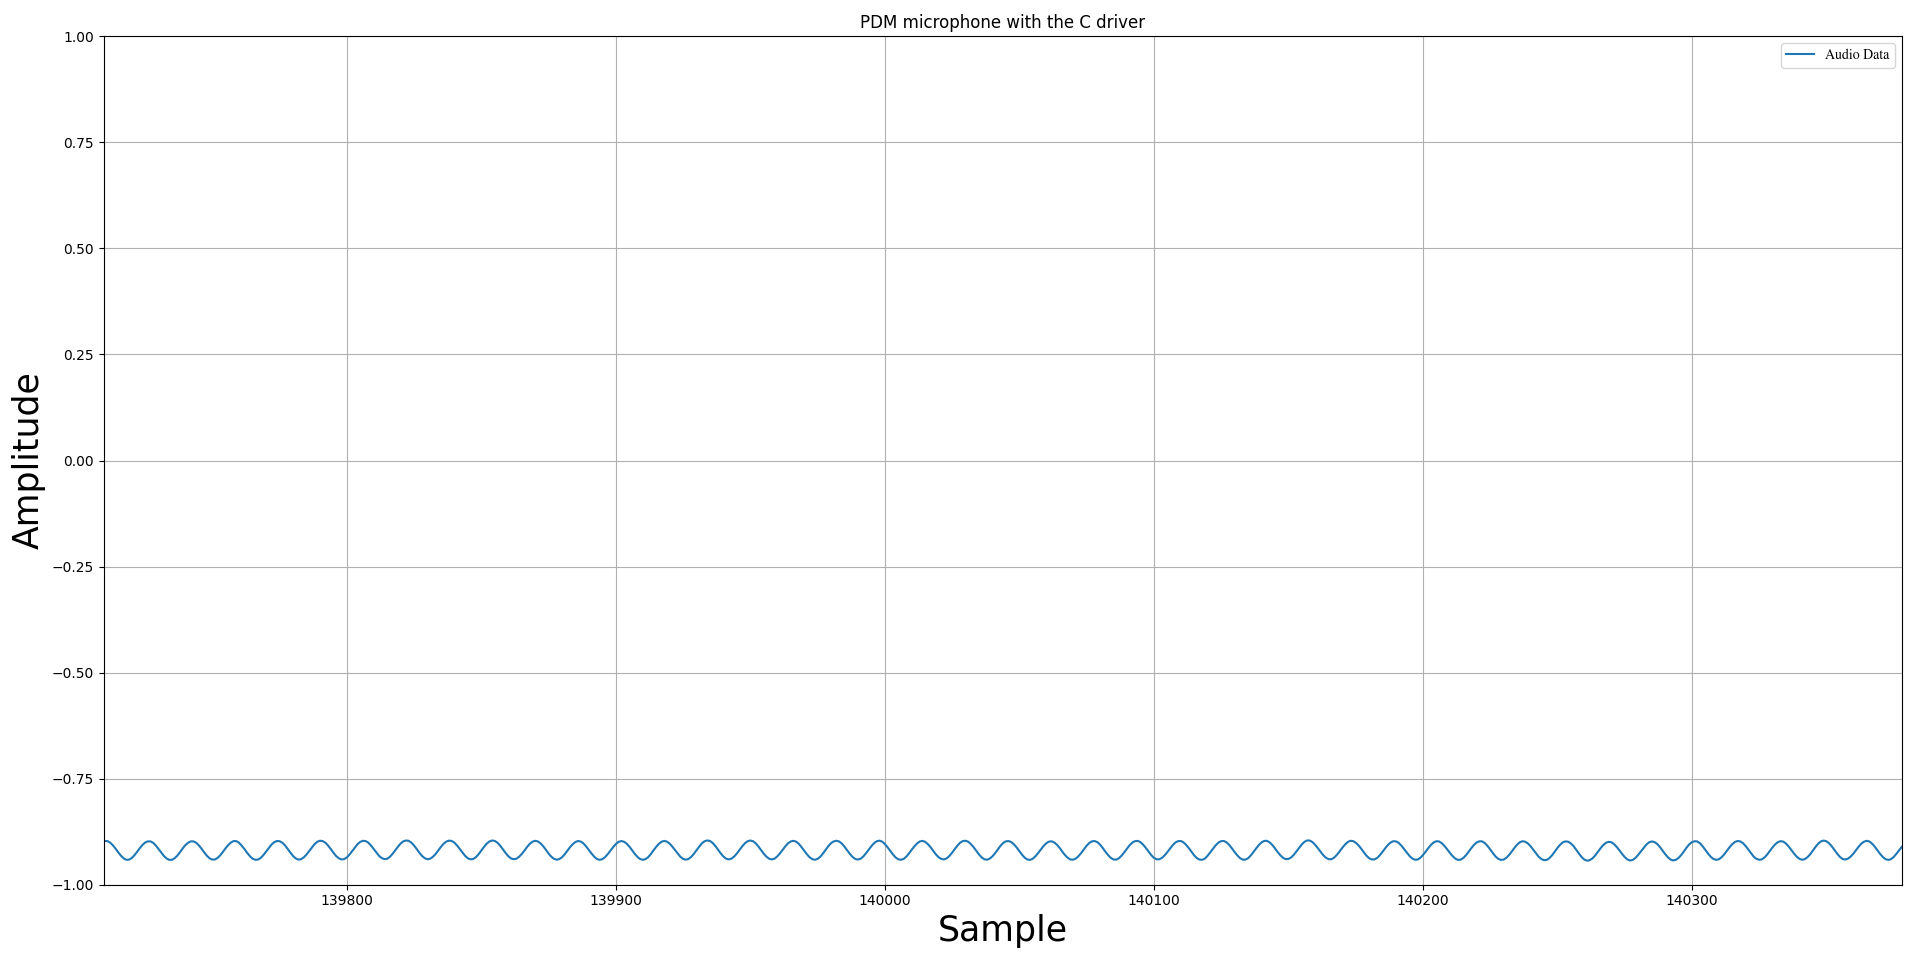
\includegraphics[width=0.9\textwidth]{figures/pdm/pdm_c.png}
    \caption[Segment of the audio data recorded by the PDM microphone using the C driver]{Segment of the audio data recorded by the PDM microphone using the C driver}
    \label{fig:pdm_c}
\end{figure}

\begin{minipage}{\textwidth}
\section{UltraTrail}

\subsection{Implementation}

To implement the driver for UltraTrail, it first has to be added to the SVD file in the PAC
as a peripheral to generate the necessary Rust code to access hardware registers.
Subsequently, the driver can be implemented in the HAL crate.
Finally, I have ported a small program from C to Rust, that contains a set of pre-defined
weights, bias and feature inputs, as well as expected results.
This program can be used to test the implementation of the driver, as it also
performs different configurations by reading and writing the different registers.
\\\\
However, there have been a few differences when it comes to the implementation details.
Most importantly, the C drivers for the PULPissimo provide the \lstinline{__rt_periph_wait_event} function,
which is basically a sophisticated busy wait.
The test code uses that function to wait for UltraTrail to trigger an event interrupt, to announce that
it is done processing as shown in Listing~\ref{code:c_wait_for_event}.
\end{minipage}

\begin{minipage}{\textwidth}
\begin{lstlisting}[style=colorEX,language=C,caption={Waiting for the event in C},label={code:c_wait_for_event}]
pacc_start();

soc_eu_fcEventMask_setEvent(ARCHI_SOC_EVENT_FCHWPE0);
__rt_periph_wait_event(ARCHI_SOC_EVENT_FCHWPE0, 1);

pacc_stop();
\end{lstlisting}
\end{minipage}

However, that function has not been implemented in the Rust drivers, so I had to slightly
vary the implementation of the test code.\\
First I had to define a Mutex \footnote{\url{https://doc.rust-lang.org/std/sync/struct.Mutex.html}}
for the event state, to monitor whether an event interrupt has been triggered as demonstrated
in Listing~\ref{code:mutex}.

\begin{lstlisting}[style=colorEX,language=Rust,caption={Definition of the necessary Mutexes},label={code:mutex}]
static EVENT_STATE: Mutex<Cell<bool>> = Mutex::new(Cell::new(false));
\end{lstlisting}

Subsequently, I defined an event handler as presented in Listing~\ref{code:event_handler}, which
stops the accelerator when it is done and changes the global event state Mutex.

\begin{minipage}{\textwidth}
\begin{lstlisting}[style=colorEX,language=Rust,caption={Event handler function},label={code:event_handler}]
fn hwpe_event_handler() {
    interrupt::free(|cs| {
        unsafe {
            Accelerator::stop_steal();
        }

        EVENT_STATE.borrow(*cs).set(true);
    })
}
\end{lstlisting}
\end{minipage}

After that I just had to enable the event and set the event handler to deal with the event when it is triggered.
The code of that can be seen in Listing~\ref{code:enable_event}.

\begin{minipage}{\textwidth}
\begin{lstlisting}[style=colorEX,language=Rust,caption={Code to enable the hardware event and set the handler},label={code:enable_event}]
unsafe {
    event_interrupt.enable_event(EventId::Hwpe0);
    event_interrupt.set_event_handler(EventId::Hwpe0, hwpe_event_handler);
}
\end{lstlisting}
\end{minipage}

Finally, I could write the busy wait, which basically does nothing until the interrupt is received
and then changes the event state.
An example of that is displayed in Listing~\ref{code:busy_wait}

\begin{minipage}{\textwidth}
\begin{lstlisting}[style=colorEX,language=Rust,caption={Snippet of the busy wait that waits for UltraTrail to finish},label={code:busy_wait}]
accelerator.start();

let mut event = false;
while !event {
    wait_x_nops(1000);

    interrupt::free(|cs| {
        if EVENT_STATE.borrow(*cs).get() {
            event = true;
            EVENT_STATE.borrow(*cs).set(false);
        }
    })
}

// ...
\end{lstlisting}
\end{minipage}

\subsection{Experiments}

The expected results are stored in a vector containing 12 16bit integers, displayed in the Listing~\ref{code:acc_results}.

\begin{minipage}{\textwidth}
\begin{lstlisting}[style=colorEX,language=Rust,caption={The expected results from the driver test},label={code:acc_results}]
let correct_results = [
    0xf246, 0x16bf, 0x08a0, 0xfe52, 0xf709, 0xef58, 0xff6b, 0xf946, 0xfebd, 0x0f40, 0xee45,
    0x18f0,
];
\end{lstlisting}
\end{minipage}

When comparing the code in Listing~\ref{code:acc_results} to the minicom output shown in \ref{code:minicom_out_acc},
one realizes that they match. Which leads me to believe that the UltraTrail driver works as intended.

\begin{minipage}{\textwidth}
\begin{lstlisting}[style=colorEx,caption={Minicom output after executing the driver test},label={code:minicom_out_acc}]
result #0: 0xf246
result #1: 0x16bf
result #2: 0x8a0
result #3: 0xfe52
result #4: 0xf709
result #5: 0xef58
result #6: 0xff6b
result #7: 0xf946
result #8: 0xfebd
result #9: 0xf40
result #10: 0xee45
result #11: 0x18f0
\end{lstlisting}
\end{minipage}

\cleardoublepage

\ifthenelse{\boolean{english}}
	{\chapter{Conclusion and Future Work}}
	{\chapter{Zusammenfassung und Ausblick}}
\label{cha:conclusion_and_future_work}
% =============================================================================
% FILE NAME : 05_conclusion_and_future_work.tex
% DEPARTMENT: University of Tuebingen
% AUTOR     : Paul Palomero Bernardo & Konstantin Lübeck
% =============================================================================
% CONTENT   : Include for chapter "Conclusion and Future Work"
% =============================================================================
Zusammenfassung der Arbeit unter Verwendung der eingeführten Begrifflichkeiten. Hier darf davon ausgegangen werden, dass der Leser die Arbeit gelesen hat bzw. kennt. Ferner sollte ein Ausblick auf Erweiterungsmöglichkeiten oder sich ergebende Forschungsfragen gegeben werden.

\cleardoublepage

\end{onehalfspace}
% =============================================================================
% Bibliography
% =============================================================================
\ifthenelse{\boolean{english}}
	{\printbibliography[title={References},heading=bibintoc]}
	{\printbibliography[title={Referenzen},heading=bibintoc]}
\cleardoublepage
% =============================================================================
% List of abbreviations
% =============================================================================
\ifthenelse{\boolean{english}}
{
	\addcontentsline{toc}{chapter}{List of Abbreviations}
	\chapter*{List of Abbreviations}
}
{
	\addcontentsline{toc}{chapter}{Abkürzungsverzeichnis}
	\chapter*{Abkürzungsverzeichnis}
}
\begin{tabbing}
\textbf{FACTOTUM}\hspace{1cm}\=Schrott\kill
\textbf{CPU}\>Central Processing Unit
\\
\textbf{GPU}\>Graphics Processing Unit
\\
\textbf{CISC}\>Complex Instruction Set Computer
\\
\textbf{RISC}\>Reduced Instruction Set Computer
\\
\textbf{SoC}\>System-on-a-Chip
\\
\textbf{PDM}\>Pulse Density Modulation
\\
\textbf{PCM}\>Pulse Code Modulation
\\
\textbf{I2S}\>Inter-IC Sound
\\
\textbf{ISA}\>Instruction Set Architecture
\\
\textbf{ML}\>Machine Learning
\\
\textbf{AI}\>Artificial Intelligence
\\
\textbf{IoT}\>Internet of Things
\\
\textbf{MSB}\>Most Significant Bit
\\
\textbf{LSB}\>Least Significant Bit
\\
\textbf{OS}\>Operating System
\\
\textbf{MCU}\>Micro-Controller
\end{tabbing}
\cleardoublepage

% =============================================================================
% List of figures
% =============================================================================
\small\normalsize
\addcontentsline{toc}{chapter}{\listfigurename}
\listoffigures
\small\normalsize
\cleardoublepage

% =============================================================================
% List of tables
% =============================================================================
\small\normalsize
\addcontentsline{toc}{chapter}{\listtablename}
\listoftables
\small\normalsize
\cleardoublepage

% =============================================================================
% "I did this myself"
% =============================================================================
\thispagestyle{empty}
\section*{Selbständigkeitserklärung}
Hiermit erkläre ich, dass ich diese schriftliche Abschlussarbeit selbständig verfasst habe, keine anderen als die angegebenen Hilfsmittel und Quellen benutzt habe und alle wörtlich oder sinngemä{\ss} aus anderen Werken übernommenen Aussagen als solche gekennzeichnet habe.
\vskip 3cm
Ort, Datum	\hfill Unterschrift \hfill
% =============================================================================
\end{document}
% =============================================================================
% DOCUMENT END
% =============================================================================
